%%% The main file. It contains definitions of basic parameters and includes all other parts.
\RequirePackage{pdf14}% also disables `\pdfobjcompresslevel`

%% Settings for single-side (simplex) printing
% Margins: left 40mm, right 25mm, top and bottom 25mm
% (but beware, LaTeX adds 1in implicitly)
\documentclass[12pt,a4paper,rgb,hyperref,table]{report}
\setlength\textwidth{145mm}
\setlength\textheight{247mm}
\setlength\oddsidemargin{15mm}
\setlength\evensidemargin{15mm}
\setlength\topmargin{0mm}
\setlength\headsep{0mm}
\setlength\headheight{0mm}
% \openright makes the following text appear on a right-hand page
\let\openright=\clearpage

%% Settings for two-sided (duplex) printing
% \documentclass[12pt,a4paper,twoside,openright]{report}
% \setlength\textwidth{145mm}
% \setlength\textheight{247mm}
% \setlength\oddsidemargin{14.2mm}
% \setlength\evensidemargin{0mm}
% \setlength\topmargin{0mm}
% \setlength\headsep{0mm}
% \setlength\headheight{0mm}
% \let\openright=\cleardoublepage

%% Generate PDF/A-2u
\usepackage[a-2u]{pdfx}

%% Character encoding: usually latin2, cp1250 or utf8:
\usepackage[utf8]{inputenc}

%% Prefer Latin Modern fonts
\usepackage{lmodern}

%% Further useful packages (included in most LaTeX distributions)
\usepackage{amsmath}        % extensions for typesetting of math
\usepackage{amsfonts}       % math fonts
\usepackage{amsthm}         % theorems, definitions, etc.
\usepackage{bbding}         % various symbols (squares, asterisks, scissors, ...)
\usepackage{bm}             % boldface symbols (\bm)
\usepackage{graphicx}       % embedding of pictures
\usepackage{fancyvrb}       % improved verbatim environment
% [round] was added manually. Use \cite{} and \citep{}
\usepackage[round]{natbib}  % citation style AUTHOR (YEAR), or AUTHOR [NUMBER]
\usepackage[nottoc]{tocbibind}
                            % makes sure that bibliography and the lists
            			    % of figures/tables are included in the table
            			    % of contents
\usepackage{dcolumn}        % improved alignment of table columns
\usepackage{booktabs}       % improved horizontal lines in tables
\usepackage{paralist}       % improved enumerate and itemize
% \usepackage{xcolor}         % typesetting in color
% \usepackage[table]{xcolor}  % typesetting in color



%%% Basic information on the thesis

% Thesis title in English (exactly as in the formal assignment)
\def\ThesisTitle{Enabling Outbound Machine Translation}

% Author of the thesis
\def\ThesisAuthor{Vilém Zouhar}

% Year when the thesis is submitted
\def\YearSubmitted{2020}

% Name of the department or institute, where the work was officially assigned
% (according to the Organizational Structure of MFF UK in English,
% or a full name of a department outside MFF)
\def\Department{Institute of Formal and Applied Linguistics}

% Is it a department (katedra), or an institute (ústav)?
\def\DeptType{Institute}

% Thesis supervisor: name, surname and titles
\def\Supervisor{doc. RNDr. Ondřej Bojar, Ph.D.}

% Supervisor's department (again according to Organizational structure of MFF)
\def\SupervisorsDepartment{Institute of Formal and Applied Linguistics}

% Study programme and specialization
\def\StudyProgramme{Computer Science}
\def\StudyBranch{General Computer Science}

% An optional dedication: you can thank whomever you wish (your supervisor, consultant, a person who lent the software, etc.)
\def\Dedication{%
I would like to express appreciation not only to my supervisor Ondřej Bojar, but also to other people who contributed to this thesis. Namely Michal Novák, Dominik Macháček and Tereza Vojtěchová (Charles University) and Frederic Blain (University of Sheffield).
Special thanks to all the people from ÚFAL with whom I spent time during my stay in the office 423 at Malá Strana.

This results of this thesis were also used for the Bergamot project which has received funding from the European Union’s Horizon 2020 research and innovation programme under grant agreement No 825303.

We used language resources developed and/or stored and/or distributed by the LINDAT-Clarin project of the Ministry of Education of the Czech Republic (project LM2010013).
}

% Abstract (recommended length around 80-200 words; this is not a copy of your thesis assignment!)
\def\Abstract{%
It is not uncommon for Internet users to have to produce text in a foreign language they have very little knowledge of and are unable to verify the translation quality. We call the task ``outbound translation'' and explore it by introducing an open-source modular system \ptakopet{}. Its main purpose is to inspect human interaction with machine translation systems enhanced by additional subsystems, such as backward translation and quality estimation. We follow up with an experiment on (Czech) human annotators tasked to produce questions in a language they do not speak (German), with the help of \ptakopet{}. We focus on three real-world use cases (communication with IT support, describing administrative issues and asking encyclopedic questions) from which we gain insight into different strategies users take when faced with outbound translation tasks. Round trip translation is known to be unreliable for evaluating MT systems but our experimental evaluation documents that it works very well for users, at least on MT systems of mid-range quality.
}

% 3 to 5 keywords (recommended), each enclosed in curly braces
\def\Keywords{%
{quality estimation}, {machine translation}, {outbound translation}, {natural language processing}, {web application}}

%% The hyperref package for clickable links in PDF and also for storing
%% metadata to PDF (including the table of contents).
%% Most settings are pre-set by the pdfx package.
\hypersetup{unicode}
\hypersetup{breaklinks=true}

% Definitions of macros (see description inside)
%%% This file contains definitions of various useful macros and environments %%%
%%% Please add more macros here instead of cluttering other files with them. %%%

%%% Minor tweaks of style

% These macros employ a little dirty trick to convince LaTeX to typeset
% chapter headings sanely, without lots of empty space above them.
% Feel free to ignore.
\makeatletter
\def\@makechapterhead#1{
  {\parindent \z@ \raggedright \normalfont
   \Huge\bfseries \thechapter. #1
   \par\nobreak
   \vskip 20\p@
}}
\def\@makeschapterhead#1{
  {\parindent \z@ \raggedright \normalfont
   \Huge\bfseries #1
   \par\nobreak
   \vskip 20\p@
}}
\makeatother

% This macro defines a chapter, which is not numbered, but is included
% in the table of contents.
\def\chapwithtoc#1{
\chapter*{#1}
\addcontentsline{toc}{chapter}{#1}
}

% Draw black "slugs" whenever a line overflows, so that we can spot it easily.
\overfullrule=1mm

%%% An environment for typesetting of program code and input/output
%%% of programs. (Requires the fancyvrb package -- fancy verbatim.)

\DefineVerbatimEnvironment{code}{Verbatim}{fontsize=\small, frame=single}



%%%
%%% Custom commands and notes
%%%

\definecolor{rubine}{rgb}{0.7, 0.1, 0.1}
\newcommand{\VVV}[1]{%
    \noindent%
    \textcolor{rubine}{VVV #1}%
}

\newcommand{\XXX}[1]{%
    \noindent%
    \textcolor{red}{XXX #1}%
}


\newcommand{\backendname}[1]{\textbf{#1}}

\newcommand{\footnotehref}[2]{%
\footnote{\href{#1}{#2}}%
}

% Hack for overfull paragraphs
\tolerance=10000
\hbadness=10000

% Figure from the img/ folder with a caption
\newcommand{\figcap}[3][1]{%
    \begin{figure}[ht]
        \centering
        \includegraphics[width=#1\textwidth]{img/#2}
        \caption{#3}
        \label{fig:#2}
    \end{figure}
}

% Multiple images per one figure
\usepackage{subcaption}

% Force figure position
\usepackage{float}

% Force footnote to stick to the bottom
\usepackage[bottom]{footmisc}

% Used for less spacing in enumerate and itemize
\usepackage{enumitem}
\setlist{noitemsep}


% multirow
\usepackage{multirow}

% Code listing environment
\usepackage{listings}
\definecolor{lightgray}{rgb}{.9,.9,.9}
\definecolor{darkgray}{rgb}{.4,.4,.4}
\definecolor{purple}{rgb}{0.65, 0.12, 0.82}
\lstdefinelanguage{TypeScript}{
  keywords={break, case, catch, continue, debugger, default, delete, do, else, false, finally, for, function, if, in, instanceof, new, null, return, switch, this, throw, true, try, typeof, var, let, string, void, while, with},
  morecomment=[l]{//},
  morecomment=[s]{/*}{*/},
  morestring=[b]',
  morestring=[b]",
  ndkeywords={class, export, boolean, throw, implements, import, this},
  keywordstyle=\color{blue}\bfseries,
  ndkeywordstyle=\color{darkgray}\bfseries,
  identifierstyle=\color{black},
  commentstyle=\color{purple}\ttfamily,
  stringstyle=\color{red}\ttfamily,
  sensitive=true
}
\lstset{
  basicstyle=\ttfamily\small,
  captionpos=b,
  language=TypeScript,
}
\lstdefinelanguage{none}{
  identifierstyle=
}
% This renames the lstlistings title
\renewcommand*{\lstlistlistingname}{List of Listings}
\renewcommand*{\lstlistingname}{List of Listings}


% 1cm hspace gap by default
\newcommand{\ttab}[1][1]{%
    \text{} \hspace{#1 cm}%
}
% cref
\usepackage[noabbrev,capitalize]{cleveref}

% Ptakopět 
\def\ptakopet{Ptakopět}


% Title page and various mandatory informational pages
\begin{document}
%%% Title page of the thesis and other mandatory pages

%%% Title page of the thesis

\pagestyle{empty}
\hypersetup{pageanchor=false}
\begin{center}

\centerline{\mbox{
\includegraphics[width=166mm]{../img/logo-en.pdf}}}

\vspace{-8mm}
\vfill

{\bf\Large BACHELOR THESIS}

\vfill

{\LARGE\ThesisAuthor}

\vspace{15mm}

{\LARGE\bfseries\ThesisTitle}

\vfill

\Department

\vfill

{
\centerline{\vbox{\halign{\hbox to 0.45\hsize{\hfil #}&\hskip 0.5em\parbox[t]{0.45\hsize}{\raggedright #}\cr
Supervisor of the bachelor thesis:&\Supervisor \cr
\noalign{\vspace{2mm}}
Study programme:&\StudyProgramme \cr
\noalign{\vspace{2mm}}
Study branch:&\StudyBranch \cr
}}}}

\vfill

% Zde doplňte rok
Prague \YearSubmitted

\end{center}

\newpage

%%% Here should be a bound sheet included -- a signed copy of the "bachelor
%%% thesis assignment". This assignment is NOT a part of the electronic
%%% version of the thesis. DO NOT SCAN.

%%% A page with a solemn declaration to the bachelor thesis

\openright
\hypersetup{pageanchor=true}
\pagestyle{plain}
\pagenumbering{roman}
\vglue 0pt plus 1fill

\noindent
I declare that I carried out this bachelor thesis independently, and only with the cited
sources, literature and other professional sources. It has not been used to obtain another
or the same degree.

\medskip\noindent
I understand that my work relates to the rights and obligations under the Act No.~121/2000 Sb.,
the Copyright Act, as amended, in particular the fact that the Charles
University has the right to conclude a license agreement on the use of this
work as a school work pursuant to Section 60 subsection 1 of the Copyright~Act.

\vspace{10mm}

\hbox{\hbox to 0.5\hsize{%
In \hbox to 6em{\dotfill} date \hbox to 6em{\dotfill}
\hss}\hbox to 0.5\hsize{\dotfill\quad}}
\smallskip
\hbox{\hbox to 0.5\hsize{}\hbox to 0.5\hsize{\hfil Author's signature\hfil}}

\vspace{20mm}
\newpage

%%% Dedication

\openright

\noindent
\Dedication

\newpage

%%% Mandatory information page of the thesis

\openright

\vbox to 0.5\vsize{
\setlength\parindent{0mm}
\setlength\parskip{5mm}

Title:
\ThesisTitle

Author:
\ThesisAuthor

\DeptType:
\Department

Supervisor:
\Supervisor, \SupervisorsDepartment

Abstract:
\Abstract

Keywords:
\Keywords

\vss}

\newpage

\openright
\pagestyle{plain}
\pagenumbering{arabic}
\setcounter{page}{1}

%%% A page with automatically generated table of contents of the bachelor thesis
\setcounter{tocdepth}{2}
\setcounter{secnumdepth}{2}
\tableofcontents

%%% Each chapter is kept in a separate file
\chapter*{Introduction}
\addcontentsline{toc}{chapter}{Introduction}

It is common for especially Internet users to have to produce text in a foreign language where they are unable to verify the quality of the proposed machine translation. The issue at hand is referred to as ``outbound translation,'' which is a complement to gisting, also known as inbound translation.

Both in gisting and outbound translation, a message is transferred between an author and a recipient. The user has sufficient knowledge of only one of the languages. In outbound translation, the user is responsible for creating correct messages, while in gisting, their responsibility is to interpret them correctly. An example of outbound translation may be filling out forms in a foreign language, describing an issue to technical support, or ordering food in a foreign restaurant. An example of gisting is to understand Internet articles, presentations correctly, or to read restaurant menus, all in a foreign language.

When translating to foreign languages, users cooperate with machine translation tools to produce the best result. Many users also use machine translation to verify their own translation, or at least to affirm, that the machine translation is valid via backward translation. Machine translation systems advanced considerably in the last decade due to breakthroughs in statistical and later neural machine translation models but they still make often mistakes. Thankfully, they are of a vastly different kind than the mistakes people make when translating texts and so are detectable.

Outbound translation is a use case, which requires some confirmation of the translation quality. Users translating to languages which they do not master enough to validate the translation could use some additional system to verify that the machine translation output is valid and assure them. This system may be the missing connection necessary for establishing trust of the user to the machine translator. We hope that MT systems will achieve perfection, but we do not expect this to happen in the foreseeable future and especially for all possible language pairs.

The issue of outbound translation has not yet been fully explored, yet there exists much research on related problems, such as quality estimation and bitext alignment, which has been productized by translation companies for minimizing post-editing costs and by other NLP companies for robust information retrieval.

The proposed tool, \ptakopet{}, aims to showcase how such a product intended to help with outbound translation may function. It provides the coveted user experience by several quality estimation pipelines and backward translation, which we hope is served in an unobtrusive, yet informative way.

We follow up with an experiment whose objective is to examine different phenomena and strategies users use with the help of \ptakopet{} when they are faced with a task involving outbound translation. Such strategies are then further examined based on their performance (relevance and quality of produced foreign texts). This experiment also gives us valuable feedback from both the user's and experiment designer's perspective. This is very beneficial to us, as we can improve the system for future experiments with \ptakopet{}.

\section*{Thesis overview}
\addcontentsline{toc}{section}{Thesis overview}
This thesis is divided into five chapters. The first one introduces terminology and issues related to machine translation, quality estimation, bitext alignment and source complexity, as well as relevant areas of research.

The second chapter covers the development and deployment of two previous versions of \ptakopet{} (old-1 and old-2) as well as what we aimed to improve and what we learned from them. We then mention different approaches to outbound translation and what we think are their positives and negatives. We also briefly discuss the industry adoption of quality estimation systems.

The next chapter shows the behaviour of \ptakopet{} from the user perspective, together with screenshots and use case descriptions.

Data preparation, experiment setup, frontend, and backend implementation, quality estimation, and bitext alignment model and deployment and usage of the current version of \ptakopet{} is the focus of the fourth chapter.

In the fifth chapter, we propose, prepare, realize, and evaluate an experiment on the strategies users take when faced with outbound translation with the help provided by \ptakopet{}. 

At the end of this thesis, we conclude and summarize both the \ptakopet{} implementation and the experiment interpretation with notes on future work in the area of outbound translation.

\chapter{Background}

This chapter aims to provide a brief overview of the available tools related to outbound translation, namely Alignment, Machine translation, Quality estimation and Source complexity.

\section{Alignment}

The alignment of parts of texts in parallel corpora is a common task in NLP and especially in tasks related to statistical machine translation. One of their use cases is creating resources used by MT systems for training. Usually, paragraph, sentence, phrase, and word alignment levels are considered. The second one and the last one are the most important for quality estimation.

A comprehensive source of alignment data is OPUS \citep{opus:2012}, which contains documents automatically aligned both on the sentence-level and word-level.

\subsection{Sentence alignment}
The task of sentence alignment is to match two groups of sentences in parallel data (usually in two languages), for example in two paragraphs or documents, if and only if they are each other's translations. A classical approach is unsupervised. In this case, the problem can be approached with a dynamic programming algorithm described by \cite{gale_church:1993}. Another approach is to view it as a machine learning problem, as summarized in \cite{yu_revisiting:2012}. Most of the approaches rely in some way on comparing the number of either, characters, words, or both in a sentence. The main idea is that a sentence's length correlates with the length of its translated counterpart.

Advances in deep neural models led to novel approaches to sentence alignment. As reported in \cite{bucc:2017}, they achieve the state of the art results. However, such models are not yet readily available for deployment.

Given a sentence alignment and a gold standard, the recall, precision and F-measure are the most common metrics.

% One of such, \cite{aghaebrahimian_alignment:2018}, achieved state-of-the-art results in BUCC 2017, as reported in \cite{bucc:2017}. 
% The sentence alignment metrics were described in depth in \cite{veronis_evaluation:2000}. 


\subsubsection{Bleualign}
Bleualign\footnotehref{https://github.com/rsennrich/bleualign}{github.com/rsennrich/bleualign} is a sentence alignment tool, which apart from the source and the target corpora requires machine translation of at least one of the texts. The alignment is then performed based on the similarity between two texts (in the target language) in the same sentence with a modified BLEU score. This approach was proposed in \cite{sennrich_bleualign:2011}.

\pagebreak
\subsubsection{Yalign}
Yalign\footnotehref{https://github.com/machinalis/yalign}{github.com/machinalis/yalign} is an open-source product of the Machinalis company. It takes a dynamic programming approach to sentence alignment, using a sentence similarity metric, which in turn utilizes SVM to tell whether a pair of sentences are each other's translations.

\subsubsection{Hunalign}
Hunalign\footnotehref{https://github.com/danielvarga/hunalign}{github.com/danielvarga/hunalign} uses the classical algorithm based on sentence-length information described in \cite{gale_church:1993}. We found it to be more robust and usable compared to other publicly available sentence alignment tools.

% It was used to build the Hunglish corpus \citep{varga:2007}, but it does not contain any Hungarian specific parts.

\subsection{Word alignment}

\begin{figure}[ht]
  \centering
  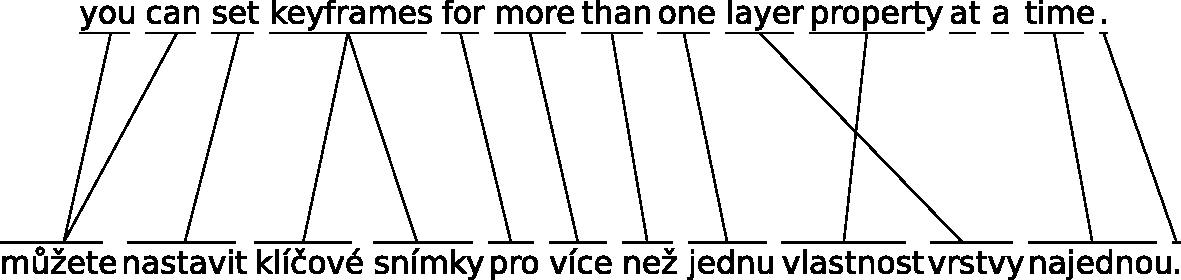
\includegraphics[width=\textwidth]{img/alignment/word_alignment_1_pdfa1a.pdf}
  \caption{\label{fig:word_alignment_1} Depiction of word alignment of the third sentence in WMT18 QE development data (English to German)"}
% You can set keyframes for more than one layer property at a time .
% Můžete nastavit klíčové snímky pro více než jednu vlastnost vrstvy najednou .
% 0-0 1-0 2-1 3-2 3-3 4-4 5-5 6-6 7-7 8-9 9-8 12-10 13-11
\end{figure}

Word alignment is the task of matching two groups of words in a bitext sentence if and only if they are each other's translations. An example\footnote{For the purposes of displaying word-alignment in the style of \cref{fig:word_alignment_1} and \cref{fig:word_alignment_2}, we wrote a small web-based tool SlowAlign. It is publicly available at \href{https://vilda.net/s/slowalign}{vilda.net/s/slowalign}. The source code is both hosted at \href{https://github.com/zouharvi/SlowAlign}{github.com/zouharvi/SlowAlign} and attached to this thesis.} of word alignment between an English sentence and translated German sentence can be seen in \autoref{fig:word_alignment_1}. Word alignment usually follows after sentence alignment.



\begin{figure}[ht]
  \centering
    \begin{tabular}{|c|c|c|c|c|c|c|}
        \hline
        & \rotatebox{90}{Klicken}
        & \rotatebox{90}{Sie}
        & \rotatebox{90}{mit}
        & \rotatebox{90}{der}
        & \rotatebox{90}{Maustaste\ }
        & \rotatebox{90}{.} \\
        \hline
        Click & \cellcolor{black} & \cellcolor{black} & \cellcolor{black} & & & \\ \hline
        the & & & & \cellcolor{black} & & \\ \hline
        mouse & & & & & \cellcolor{black} & \\ \hline
        button & & & & & \cellcolor{black} & \\ \hline
        . & & & & & & \cellcolor{black} \\ \hline
    \end{tabular}
  \caption{\label{tab:word_alignment_2} Bitext matrix of English to German word alignment}
\end{figure}

Sometimes the word alignment is depicted as in \cref{tab:word_alignment_2}, which is known as a bitext matrix. There is a point on $A_{i,j}$ if and only if the $i-$th source word is aligned to the $j-$th target word. Diagonal bitext alignment would correspond to a bitext matrix with points on its diagonal (a geometrical diagonal for non-square matrices). Sometimes it is impossible to do word alignment. Example of this are idiomatic phrases, whose translations can be idiomatic phrases in the target language and then there is no explicit mapping between individual words. We show such an example of only a partial matching in \cref{fig:word_alignment_2}. In this case using phrase-level alignment may be more suitable, as explored in \cite{bojar-prokopova:phrasal}. However, for most cases, we are able to construct meaningful word-level alignment.

\begin{figure}[ht]
  \centering
  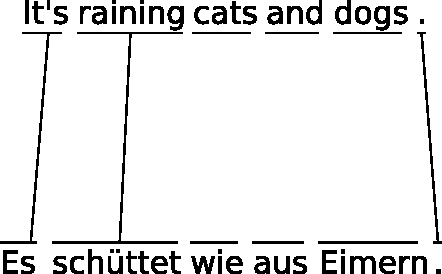
\includegraphics[width=0.36\textwidth]{img/alignment/word_alignment_2_pdfa1a.pdf}
  \caption{\label{fig:word_alignment_2} A partial alignment of an English idiom and its corresponding German translation.}
% It's raining cats and dogs .
% Es schüttet wie aus Eimern .
% 0-0 1-1 5-5
\end{figure}

For a long time, increasingly complex IBM Alignment Models 1 to 6 dominated the area of word-level alignment.\footnotehref{http://www.statmt.org/survey/Topic/IBMModels}{statmt.org/survey/Topic/IBMModels}  These models are a coproduct of statistical machine translation models. Summary of the development of IBM word alignment models can be found in the second chapter of \cite{cuvrin_alignemnt:2006}.

% There are two approaches to statistical word alignment. 
% Models 2 and 3 fix certain pitfalls of model 1. These improvements are penalization of translated words that are out of position and modelling probability of one word being translated into $n$ others. Model 3 implements a better solution to the fertility problem (modelling probability of an insertion). Model 4 introduced taking previously aligned words into account, while model 5 further refines this concept by penalizing the placement of two words in the same position. All of these five models were described in \cite{brown_ibm_1_2_3_4_5:1993}.  Model 6, the last model, stands out by combining model 4 with an alignment model based on Hidden Markov Models by \cite{vogel_hmm:1996}. 

Similarly to sentence alignment, research in the area of neural networks allowed for state-of-the-art results. An example of this can be found in \cite{legrand:2016}, where the authors use the dot product of windows from two convolutional layers (source and target) as the alignment score. As far as we know, none of the neural models has been made into a deployable word alignment tool. There are however hints of progress, as word alignment can be extracted from neural attention based machine translation systems, shown in Nizza\footnotehref{https://github.com/fstahlberg/nizza}{github.com/fstahlberg/nizza} and Neural Machine Translation.\footnotehref{https://github.com/tilde-nlp/neural-machine-translation-tools}{github.com/tilde-nlp/neural-machine-translation-tools}

The task of word alignment is formalized in \cite{mihalcea_evaluation:2003} together with four standard metrics: precision, recall, F-measure and quality of word alignment.

\pagebreak
\subsubsection{GIZA, GIZA++, MGIZA++, PGIZA++}
The GIZA word alignment collection is a standard used for this task. The first version, GIZA, was part of the EGYPT SMT toolkit and was later extended to GIZA++ and later became part of the Moses SMT toolkit.\footnotehref{http://www.statmt.org/moses/}{statmt.org/moses/}  It incorporates IBM Model 4, IBM Model 5 and Hidden Markov Models. The support for multithreading and clusters was later added, resulting in MGIZA++\footnotehref{https://github.com/moses-smt/mgiza}{github.com/moses-smt/mgiza} and PGIZA++\footnotehref{http://www.cs.cmu.edu/~qing/giza/}{www.cs.cmu.edu/\~qing/giza/}, respectively.

% It was presented in \cite{gizapp:2003}

In addition to word alignment, all of the ++ versions can perform some rudimentary form of sentence alignment.

\subsubsection{Fast\_align}
Fast align \citep{fastalign:2013} is a word aligner based on IBM Alignment Model 2, with improvements on this model's over-parametrization issues. It outperforms the commonly used IBM Alignment Model 4, is easy to build and use and has low resource requirements (both memory and computational time). It is often used as a baseline solution.

\subsubsection{Eflomal}
Eflomal\footnotehref{https://github.com/robertostling/eflomal}{github.com/robertostling/eflomal} is an improved version of Efmaral presented in \cite{ostling_efmaral:2016} together with comparison to the other two-word alignment systems. It is based on Bayesian alignment models with Markov Chain Monte Carlo inference. It is currently the state-of-the-art in word alignment.

\section{Machine translation}

The task of machine translation is to translate text from one language to another. In this context, it is strictly automatic and should not be confused with machine-aided human translation. This is an extensive topic and beyond the scope of this thesis. We thus provide only a very brief overview of the evolution and main approaches.

\subsection{Rule based (RBMT)}

First attempts for machine translation were made with rule-based systems, with either direct, syntactic or semantic transfer, which corresponds to steps described by the Vauquois triangle.\footnotehref{http://mttalks.ufal.ms.mff.cuni.cz/index.php?title=Intro\#Types\_of\_MT\_systems}{mttalks.ufal.ms.mff.cuni.cz/index.php?title=Intro\#Types\_of\_MT\_systems} Models based on the manipulation of morphological, syntactic and semantic structures are known as transfer based. They require linguistic knowledge of both source and target languages to be produced. We list examples of RBMT systems with short descriptions. Most of them became obsolete with the advent of statistical machine translation systems.

\begin{itemize}
    \item Ruslan - Created for Czech-Russian translation \citep{ruslan}.
    \item APAČ - Created for Czech-English translation \citep{apac}.
    \item METEO - Used for 20 years for English-French Canada weather reports translation \citep{meteo}.
    \item SYSTRAN - Developed by one of the oldest companies providing MT. It supports many language pairs and transitioned to SMT and NMT later \citep{systran}.
\end{itemize}

\subsection{Statistical (SMT)}
\label{subsec:smt}

Statistical machine translation models rely on a great amount of parallel data. They are usually modelled with two components: translation model and language model. This is shown in \autoref{eq:language_bayes} which shows the common application of the Bayes theorem for best translation $t$ given a source sentence $s$. The model is split into the translation model $p(s|t)$, evaluating translation relevance, and language model $p(t)$, which describes how well the proposed target sentence fits the language. The motivation is that monolingual data, used by the language model, are much easier to obtain than bilingual ones.

\begin{equation}
    \text{argmax}_t\ p(t|s) = \text{argmax}_t\ \frac{p(t)\cdot p(s|t)}{p(s)} = \text{argmax}_t\ p(s|t)\cdot p(t)
    \label{eq:language_bayes}
\end{equation}

The language model is usually modelled with n-grams. Its use made the translations more fluent as opposed to previous approaches.

SMT was first word-based, meaning words were manipulated and strung together to form a sentence. An example of this are the IBM models \citep{brown_ibm_1_2_3_4_5:1993}. More modern systems were phrase-based (documented in \citep{koehn2003statistical}), meaning whole sequences of words were manipulated and composed to form a sentence. This approach was widely adopted in the industry. We list examples of MT systems which are or were SMT based.

\begin{itemize}
    \item Google Translate - Is one of the most known publicly available MT system.\footnotehref{https://www.blog.google/products/translate/ten-years-of-google-translate/}{blog.google/products/translate/ten-years-of-google-translate/} It started transitioning to NMT in 2016.\footnotehref{https://www.blog.google/products/translate/found-translation-more-accurate-fluent-sentences-google-translate/}{blog.google/products/translate/found-translation-more-accurate-fluent-sentences-google-translate/}
    \item Bing Translator - Developed by Microsoft and is another widely used publicly available MT. It started transitioning to NMT in 2016.\footnotehref{https://www.microsoft.com/en-us/translator/business/machine-translation/}{microsoft.com/en-us/translator/business/machine-translation/}
    \item SYSTRAN - Was SMT, but partially transitioned to NMT in 2016.\footnotehref{http://kv-emptypages.blogspot.com/2016/12/systrans-continuing-nmt-evolution.html}{kv-emptypages.blogspot.com/2016/12/systrans-continuing-nmt-evolution.html}
\end{itemize}

\subsection{Neural (NMT)}

In the past decade, NMT systems became the state of the art and thus widely used. There are two main cornerstones of NMT: encoder-decoder and (self-)~attention. They both rely on recent advances in representation learning.

\subsubsection{Embedding}
One possibility to represent words in memory is using one hot encoding. Given a dictionary $D$, the $i$-th word of the dictionary would be represented by a vector of size $|D|$ of zeros except for one $1$ in the $i$-th place. This is far from the optimal approach, and there are many associated issues, such as data sparsity. In this encoding, each word form would be equally distant from each other. So the difference between the embeddings of \texttt{birds} and \texttt{bird} would be the same as between the embeddings of \texttt{birds} and \texttt{refrigerated}.

An alternative to this is to make a neural network learn a word representation. In this context, the representation is named \textit{word embedding}. Word2Vec \citep{word2vec} are types of networks, which can create such word embeddings out of monolingual data in an unsupervised way.
The authors propose two architectures. The first one is Continuous Bag-Of-Words, which tries to predict the current word based on the context, and the other is Skip-Gram, which tries to predict the context based on the current word. 
% \footnote{The tokens in the data are actually in sequence and not just a set. So the context of the word is the supervision.}

Word embeddings are able to capture relationships between embedded words. So word embeddings for \texttt{birds} and \texttt{bird} would be closer together than the word embeddings for \texttt{birds} and \texttt{refrigerated}.

Another improvement was the introduction of subword units and relevant training algorithms, such as Byte Pair Encoding \citep{subwords_bpe}. Subword units are used to deal with unseen and rare words. If a word is too rare, it will not get its own word embedding but will be split into multiple subword units. This is intuitive, as humans are able to understand new words by analyzing their morphemes.

\subsubsection{Encoder-Decoder}
The encoder-decoder architecture is the standard approach for sequence to sequence tasks. In this case, it is a sequence of word embeddings, which is passed to multi-level bidirectional RNN, composed of either Long Short Term Memory (LSTM) or Gated Recurrent Unit (GRU). The result is called the hidden state, and it is a fixed-size vector, which is passed between the cells. The hidden state represents the whole input sentence. To get the translated output, the hidden state is unrolled with the same mechanism, but this time the probabilities of all possible output subword units are produced. A search algorithm, possibly a greedy one, selects one of them and the decoder moves to the next step.


% word embeddings are outputted. They are then mapped to subword units (with target embedding) and form the output sentence. 



The actual recurrent neural networks used for machine translation are made more complex, such as with the use of multiple layers of encoders.

\subsubsection{Attention}

One of the deficiencies of the purely encoder-decoder approach is that both of the RNN components only have direct access to the immediately preceding word. This is a problem in case the translation of the current word is dependent on a word, which was either encountered (source) or generated (target) several steps back. Such distant word is embedded in the hidden state (fixed size vector), but it may be too difficult to extract its features.

A novel approach was taken by \cite{bahdanau2014neural}. They proposed a system by which a current (to be produced) word can reference the words the translation is dependent on. Such referencing is called the attention mechanism and there are two types usually distinguished: global attention and local attention. This mechanism is employed only in the decoder part and the attention mechanism adds a context vector to the word translation computation.

Global attention computes the context from all of the source words using a hidden alignment vector, which supplies weights for each word. Local attention focuses on a window of a fixed size around the aligned source word.

Popular MT models such as Transformer \citep{attention_all_you_need} or BERT \citep{bert} make use of attention mechanisms and add other improvements, such as multi-head self-attention. As is apparent from the transition in the industry standard in the listing in \cref{subsec:smt}, NMT together with attention mechanisms outperforms SMT and it is now the state of the art and widely used.

\subsection{Evaluation}

Automatic machine translation evaluation assigns scores to the produced machine translations, given also the source text and reference translation. The goal is to find such a metric, that would correlate the most with human annotations. This is not an easy task to automate, as the machine translation can be vastly different from the reference translation, but still be correct. Alternatively, it can be very close to the reference translation, but be very ungrammatical or can distort the meaning seriously.

Many other metrics have been proposed and this area of research is still active. The metrics shared task is part of WMT \citep{wmt19_metrics}.

\subsubsection{BLEU}
Bilingual Evaluation Understudy \citep{bleu} is the most common metric for evaluation of MT systems. It is based on searching for n-grams in the translated sentence, which are also in the reference translation. The geometric mean of unigram, bigram, trigram and quadrigram precision is calculated and the score computed as in the formula in \cref{fig:bleu}. 

The first part of the product is called the \textit{brevity penalty}. It is there to make sure that the MT system does not game the metric by outputting for example only one quadrigram, which it is very sure about. In this case all of the precisions would be close to $1$, but human annotators would not consider this to be a good translation.

\begin{equation}
    \text{BLEU} = exp\big(\min(1, 1-\frac{\text{output length}}{\text{reference length}})\big) \cdot \big(\prod_{i=1}^4 \text{prec}_i\big)^\frac{1}{4}  
    \label{fig:bleu}
\end{equation}

\subsubsection{METEOR}
Metric for Evaluation of Translation with Explicit ORdering aims to fix some disadvantages of BLEU. In contrast to BLEU, it considers only unigrams and not bigrams, trigrams, nor quadrigrams. It uses stemming and synonyms and tries to create mappings between the translated and reference sentence. It has been shown \citep{meteor} that it correlates better with the human judgement than BLEU.

\subsubsection{Round trip translation}

Also called backward translation, round trip translation is an idea of evaluating an MT system without reference. It is based on translating the source sentence to a foreign language and then back and measuring BLEU score between source and backward translated text. In \citep{rtt_what_is_it_good_for} it was demonstrated, that RTT does not correlate with the quality of MT systems in any statistically meaningful way.

\section{Quality estimation}
As opposed to machine translation evaluation, which uses source text and target and reference translations to evaluate the output, the objective of quality estimation (also known as confidence estimation) is to predict the translation quality without reference translations.

Machine translation quality estimation aims to provide hints as to whether a produced machine translation is good or bad. Quality estimation shared task was part of WMT since 2012\footnotehref{http://www.statmt.org/wmt12/quality-estimation-task.html}{statmt.org/wmt12/quality-estimation-task.html} and was forked from automatic machine translation evaluation shared task, which was part of WMT since 2008\footnotehref{http://www.statmt.org/wmt08/shared-evaluation-task.html}{statmt.org/wmt08/shared-evaluation-task.html} and in 2012 renamed to metrics task. The results of the latest findings of the WMT quality estimation shared task 2019 are discussed in \citep{wmt_qe:2019}.

The input of metrics task, as defined by WMT, is the translation together with human reference translations. It is performed usually on sentence-level and system-level. In contrast, the input for quality estimation system is the source text and the translated text. Quality estimation is then performed on word-level, phrase-level and sentence-level.

For document-level quality estimation, the document is either to be assigned a score, or the system should report spans, which contain translation errors. The quality of sentence-level quality estimation is measured in HTER (edit-distance metrics).


The output of word-level quality estimation is usually a list of probabilities for each token in the target sentence. In WMT, the format is only binary values for each token. For word-level quality estimation models, to encapsulate missing words, tokens for gap were added. Thus each space adjoining a target token can also be classified as \texttt{OK} or \texttt{BAD}, denoting a missing word in the latter case. For $N$ target tokens, $2\cdot N + 1$ binary values should be generated. This is illustrated in \autoref{fig:word_level_gaps}.

\begin{figure}[ht]
  \centering
  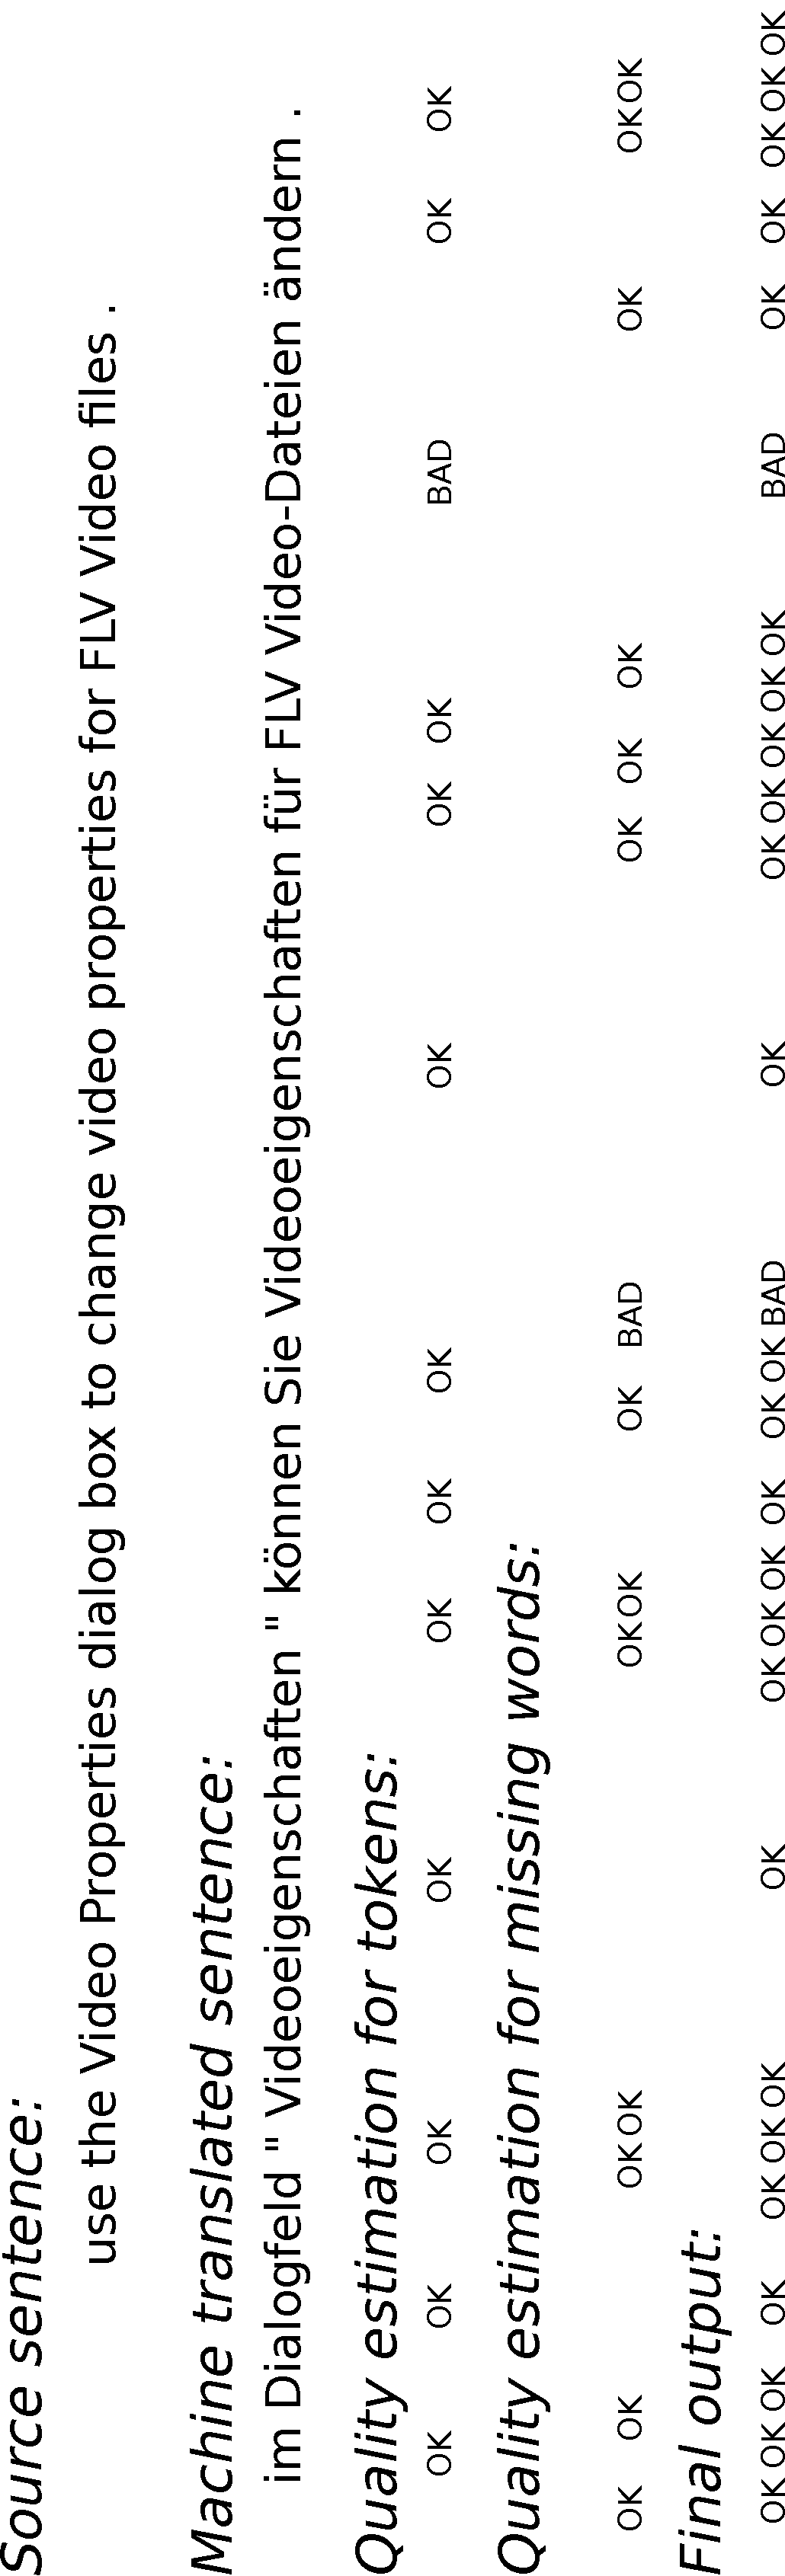
\includegraphics[height=\textwidth, angle=-90]{img/quality_estimation/format_pdfa1a.pdf}
  \caption{\label{fig:word_level_gaps} Quality estimation tags for tokens and gaps on German sentence translated from English (from WMT19 quality estimation shared task)}
\end{figure}

\pagebreak
\subsection{QE from machine translation models}
Some machine learning systems, especially classifiers, are able to report also the confidence in their output. To our knowledge, quality estimation from the machine translation models themselves is used only in combination with another QE system which use this self-reported confidence as one of the features.

\subsection{QuEst++}
The main pipeline of QuEst++ by \cite{questplusplus} consists of feature extraction and machine learning prediction. This system first extracts features from the input data and then runs a machine learning algorithm for example with scipy's LarsCV (Cross-validated Lasso, using the LARS algorithm) or Conditional Random Fields suite by \cite{CRFSuite}.

A large part of their work is devoted to feature exploration and fine-tuning. There are four groups of features for word-level quality estimation:

\begin{itemize}
    \item word alignment
    \item POS of source and target words
    \item n-gram frequencies in source and target texts
    \item syntactic, semantic and pseudo-reference binary flags
\end{itemize}

They are an extension of features for word-level quality estimation used by WMT12-13-14-17-18 for the baseline model.\footnotehref{https://www.quest.dcs.shef.ac.uk/quest\_files/features\_blackbox\_baseline\_17}{quest.dcs.shef.ac.uk/quest\_files/features\_blackbox\_baseline\_17} For sentence-level, the features are focused on the relations of tokens in the source and target sentences, e.g. the ratio of such tokens and distribution of parts of speech. Document features incorporate aggregation of sentence-level features as well as features on the discourse level by \cite{scarton_reading:2016}.

Since the system was not designed to provide online results, the consequence is, that especially the feature extraction part is not optimized and is quite slow. It can handle only ten sentences at a time, so larger inputs have to be split into multiple batches. At the time of deployment there were two bugs, for which we opened pull requests.\footnote{\href{https://github.com/ghpaetzold/questplusplus/pull/45}{github.com/ghpaetzold/questplusplus/pull/45} and \\ \ttab[0.5] \href{https://github.com/ghpaetzold/questplusplus/pull/46}{github.com/ghpaetzold/questplusplus/pull/46}}


\subsection{DeepQuest}
DeepQuest \citep{deepquest} takes a neural approach to quality estimation and is capable of performing on any language pair. The toolkit offers two architectures.

\begin{figure}[H]
  \centering
  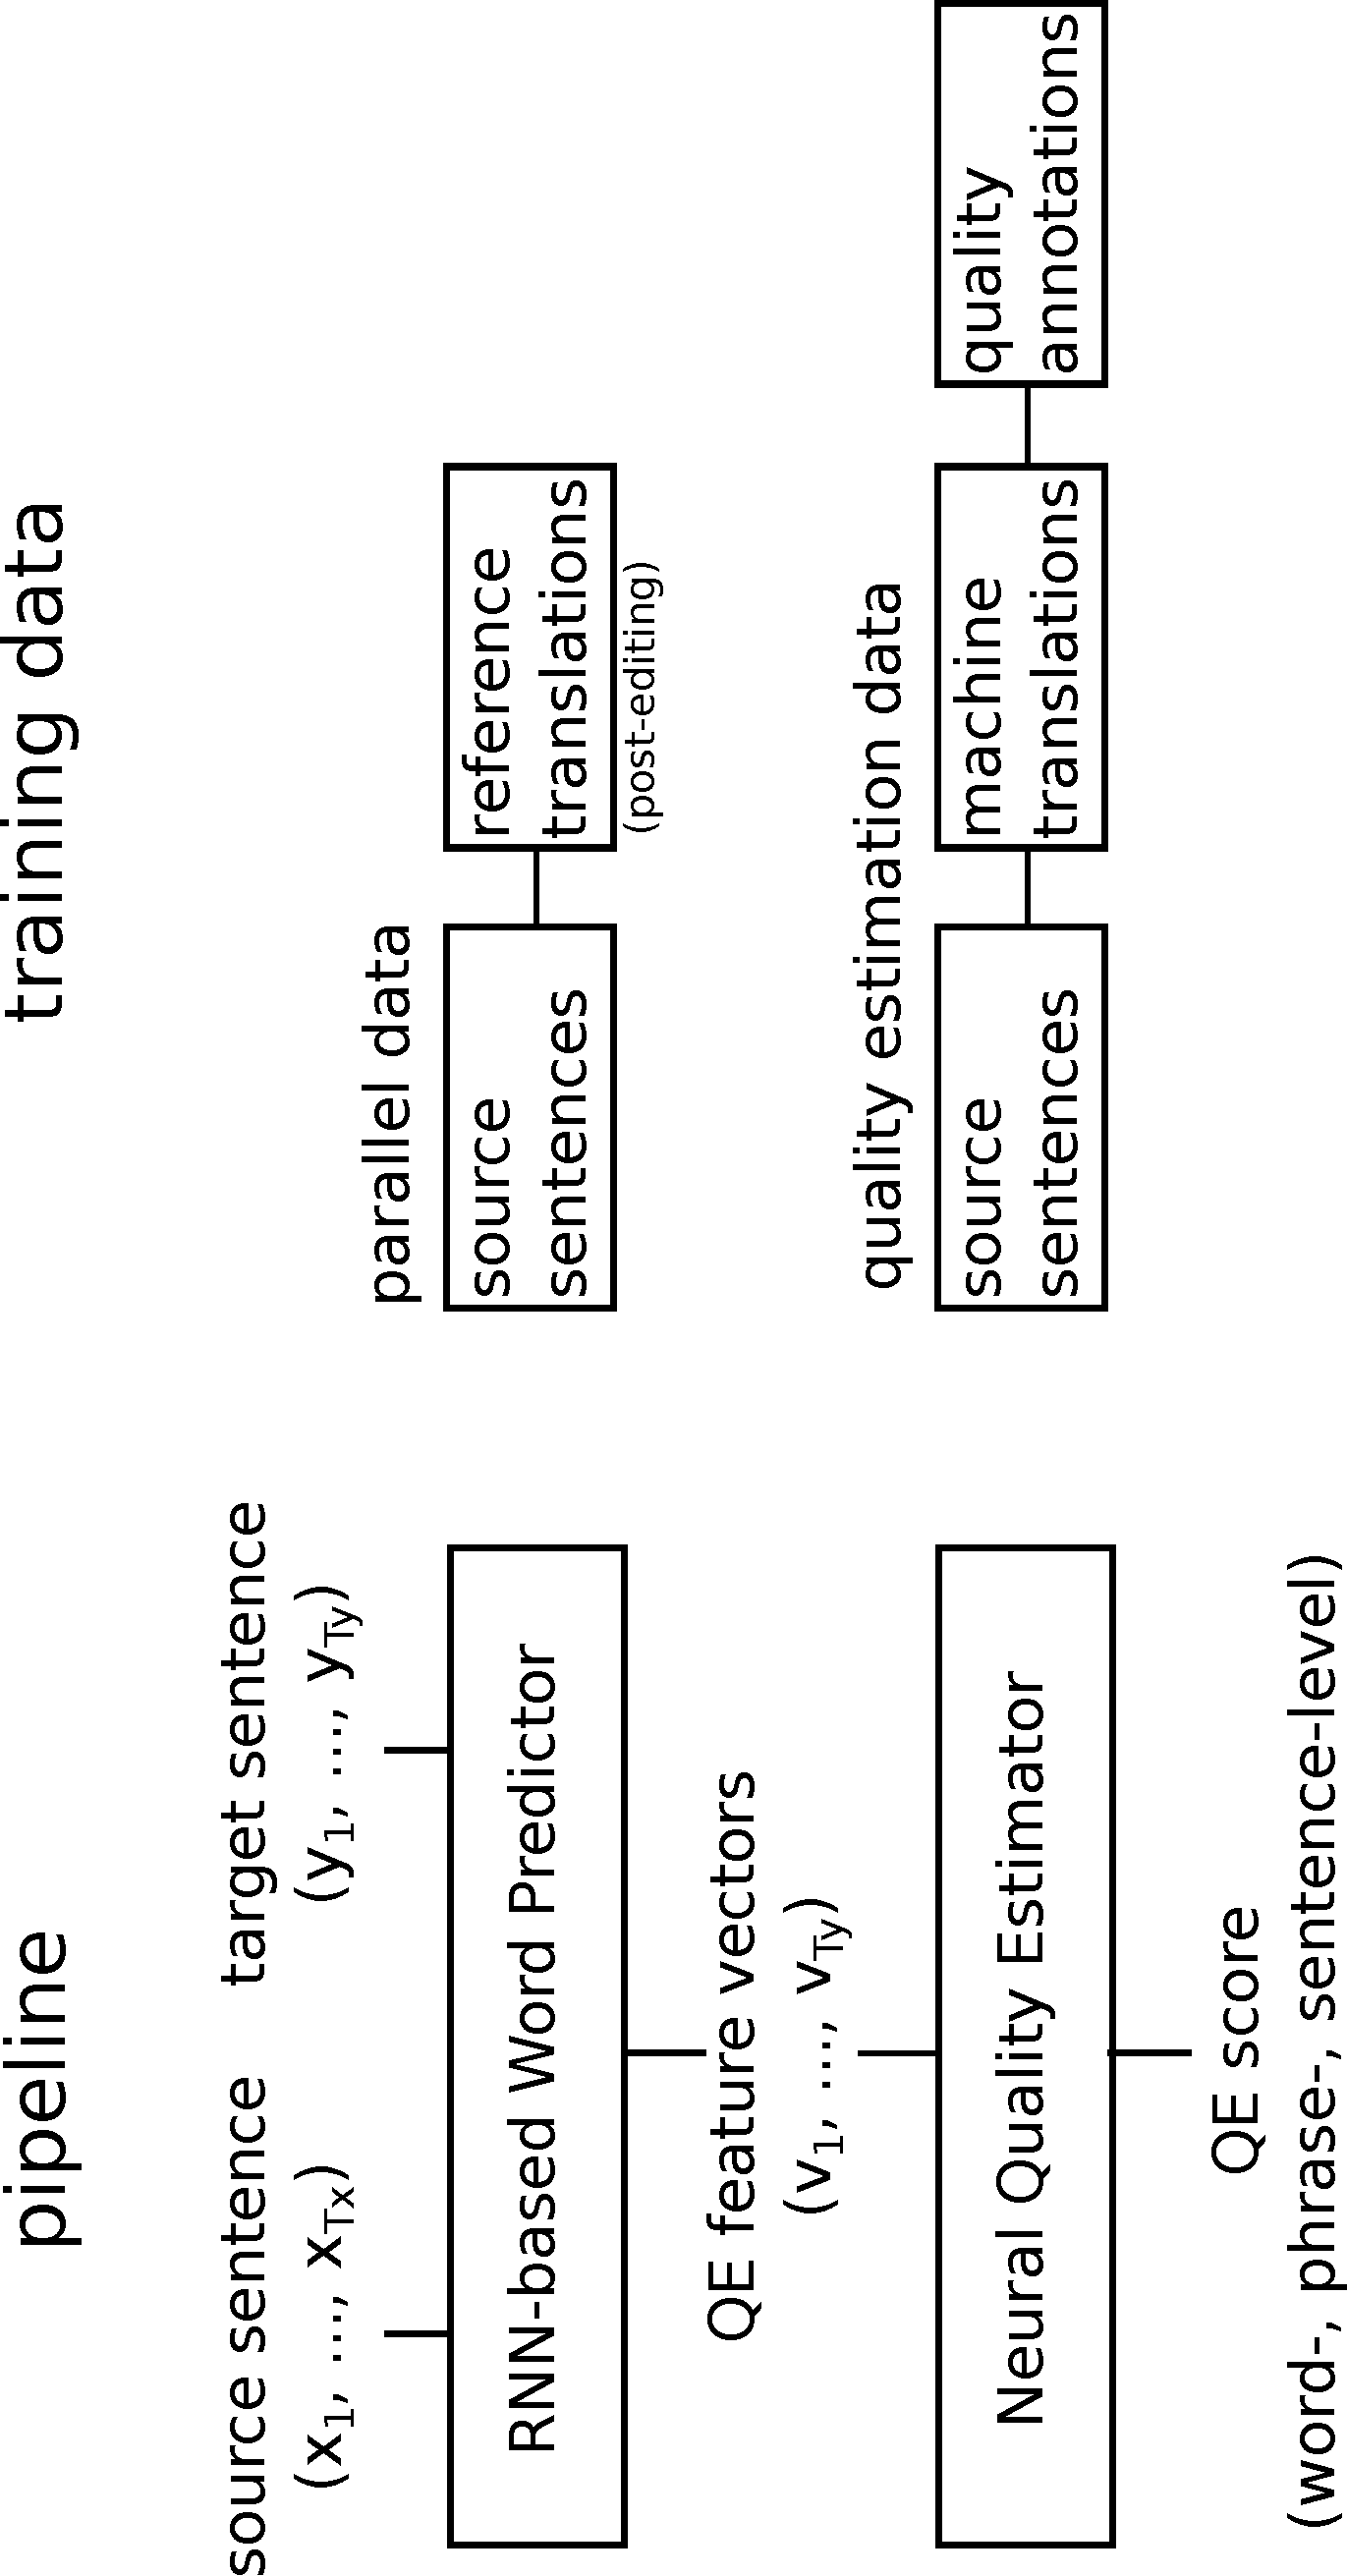
\includegraphics[height=0.9\textwidth, angle=-90]{img/quality_estimation/postech_architecture_pdfa1a.pdf}
  \caption{\label{fig:postech_architecture} Predictor-Estimator QE model pipeline and type of training data, adapted from Fig. 1 from \citep{Kim-Postech:2017}}
\end{figure}

Predictor-Estimator architecture \citep{Kim-Postech:2017} consists of two stages of training. In the first one, a predictor (encoder-decoder RNN) is trained on parallel data to predict words based on their context representations. Feature vectors from this network are then passed to the estimator, which is trained on quality estimation data. This delegates the issue of feature engineering onto machine learning itself. The architecture is illustrated in \autoref{fig:postech_architecture}.

The other architecture implemented by DeepQuest is biRNN. A sequence is passed into RNN both in the original ordering as well as in reverse. The results are then concatenated and propagate further into the rest of the network. The network can then make use of not only the preceding item in the sequence but also the subsequent one.

Models of both architectures can be executed on document-level, sentence-level, phrase-level and word-level.

\cite{deepquest} reported better results in most experiments on WMT17 with the Predictor-Estimator than the baseline (QuEst++). Performance of the biRNN architecture is still better than the baseline and does not significantly lack behind the Predictor-Estimator. They also stress the difference of performance of implemented systems on SMT and NMT data, with the later resulting in worse results, presumably because the error is less predictable in the latter case.

Despite the better results, we found the implementation difficult to work with because of several bugs. Even though some of the bugs we reported were fixed, the latency of this tool was still too high for online purposes.

\subsection{OpenKiwi} \label{subsec:openkiwi}

OpenKiwi \citep{openkiwi} implements three quality estimation models: QUality Estimation from ScraTCH \citep{kreutzer-quetch:2015}, NeUral Quality Estimation \citep{martins-unbabel:2016} used for WMT19\footnotehref{http://www.statmt.org/wmt19/qe-task.html}{statmt.org/wmt19/qe-task.html} baseline and Predictor-Estimator \citep{Kim-Postech:2017}. In addition OpenKiwi implements stacked ensemble as proposed in \cite{martins-ms:2017}.

QUETCH is a linear combination of baseline features and custom neural network. The architecture of the later is shown in \autoref{fig:quetch_architecture}. For each target token $t_i$ an aligned source token $s_{a(i)}$ is considered. Then windows of size three are concatenated: $(t_{i-1}, t_i, t_{i+1}, s_{a(i)-1}, s_{a(i)}, s_{a(i)+1)}$ and passed through a lookup-table (pretrained word2vec). The resulting vectors are then passed through a densely connected layer and finally through an output layer, which outputs \texttt{OK} or \texttt{BAD}.

\begin{figure}[ht]
  \centering
  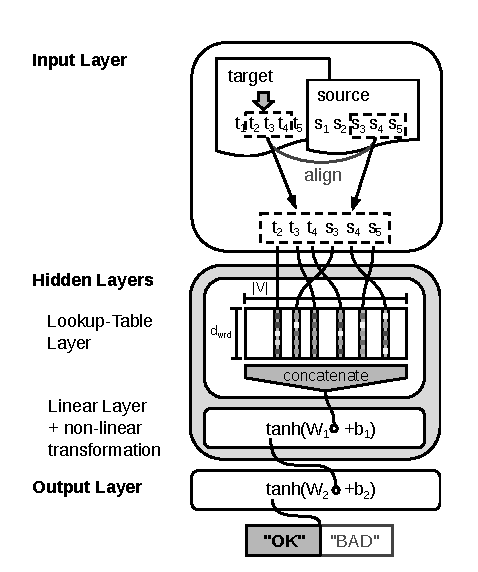
\includegraphics[width=0.6\textwidth, angle=0]{img/quality_estimation/quetch_architecture_pdfa1a.pdf}
  \caption{\label{fig:quetch_architecture} QUETCH model architecture, from Fig. 1 in \citep{kreutzer-quetch:2015}}
\end{figure}

NuQE is very similar to QUETCH in most respects. In addition, POS tags are concatenated and passed through a POS embedding table and finally, two layers bidirectional gated recurrent units are appended (with two extra dense layers in between).

We opted for the Predictor-Estimator architecture because even though it requires pretraining, it does not consume many resources compared to the stacked ensemble. Except for the ensemble, it also provides the best results as shown in \cite{openkiwi}. OpenKiwi, in general, proved to be faster, more robust and easier to use\footnote{OpenKiwi is distributed via pip \href{https://pypi.org/project/openkiwi/}{pypi.org/project/openkiwi/} as a Python module.} than DeepQuest. Because of this, the experiment was conducted with this quality estimation backend.

\subsection{Evaluation}

Since the output of sentence-level and phrase-level quality estimation is usually HTER, there are several metrics for quality estimation systems. They are measured over the whole dataset.

\begin{itemize}
    \item Root Mean Squared Error
    \item Mean Average Error
    \item Pearson's correlation
    \item Spearman's rank correlation
\end{itemize}

For word-level quality estimation, the output is a sequence of probabilities, which can be, for a given threshold, transformed into a sequence of two classes \texttt{OK} and \texttt{BAD}. Since the distribution of \texttt{OK} and \texttt{BAD} for most of the sentences is unbalanced, accuracy could be cheated by predicting always \texttt{OK}. To balance precision and recall, F measure with respect to \texttt{OK} and \texttt{BAD} is used. To incorporate both, $F_{MULTI} = F_{OK}\cdot F_{BAD}$ is usually used as a metrics for WMT quality estimation task.

\section{Source complexity}

The task of estimating source complexity is not rigidly defined and has not been thoroughly explored. In the context of machine translation, we can think of it as finding patterns in a sentence which are hard to translate by MT systems. For our purposes, it is beneficial to know which parts of the source sentence are challenging to translate, so that users speaking only the source language can reformulate that specific segment.

\subsubsection{Lexical choice}

One of the most straightforward ideas would be to look at individual words in the source sentence and describe the probability of them being translated correctly. This can be done, for example, by searching for that word in the data the specific MT system used for training. Subword units can help with unseen words, but we can still hypothesize, that if a word has never been seen by an MT system, it will be difficult to translate.

Another approach to recognize problematic source words would be using word alignment and word-level quality estimation. A QE system gives a score to every translated word. These values can be mapped back to the source sentence by word alignment. This approach was chosen for \ptakopet{} because it could be done with already existing tools. The implementation is discussed in \cref{subsubsec:impl:source_complexity}.

\pagebreak
\subsubsection{Syntactic structures}

For most MT systems it is not a single unknown word which worsens the translation quality but syntactic structures. This has been described extensively in \cite{choshen_challenge_sets}. Their claim is that long distance dependencies are still a massive problem for translation quality.

The work of \cite{niehues_confidence} focuses not only on target tokens QE but also on confidence annotation of source tokens. Their methods are based on complex similarity measures between the given source sentence and training data.
\chapter{Previous work}

This thesis is focused on the latest version of \ptakopet{}. The previous two versions (old-1 and old-2) were vastly different and created as part of two other classes taught at Charles University. Summaries of their respective goals, functionalities, and conclusions follow. Both projects are archived in a combined GitHub repository.\footnotehref{https://github.com/zouharvi/ptakopet-old}{github.com/zouharvi/ptakopet-old}

We also comment on the adoption of quality estimation systems in the industry and publicly available services \cref{sec:related_industry}.

\section{\ptakopet{} old-1}

\subsection{Introduction}
The first version was developed as a semestral assignment for class Competing in Machine Translation led by Ondřej Bojar. The goal was to explore the issue of outbound translation for daily internet usage (e.g. filling out forms in websites of a foreign language). Because of this intended usage, it was designed as a browser extension compatible with major browsers (tested on Firefox, Google Chrome, and Opera).

It used to be available on Chrome Web Store and Add-ons for Firefox, but we removed it from these places as this version soon became deprecated.

\subsection{Usage}

The core functionality was to display backward (round-trip) translation so that users could check, for example, whether the verb tense was changed or if the backward translation matches the original sentence in its meaning. This basic functionality, which remained in future version, gave this project the name of \ptakopet{} (\textbf{p}řeklad \textbf{t}am \textbf{a} \textbf{ko}ntrolně z\textbf{pět}).
\ptakopet{} old-1 ran as a small plugin located, if active, in the top left or top right corner of the page. The plugin could be used either as a browser extension (users install this extension) or as a part of a web page (web admin inserts a loading script into their page).

\begin{figure}[ht]
    \centering
    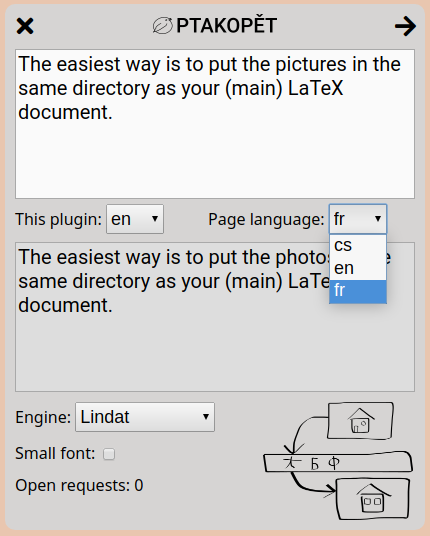
\includegraphics[width=0.6\textwidth]{img/ptakopet_old-1/lang_select}
    \caption{User interface of the \ptakopet{} old-1 browser extension}
    \label{fig:ptakopet_old-1/lang_select}
\end{figure}

The plugin shown in \cref{fig:ptakopet_old-1/lang_select}, contains two main textareas. The top one expected input in the language of the user. The bottom one eventually contained the backward translation. The translation was in the active input element (on the webpage). This process of three text elements (input, translation and backward translation) was hard to communicate to users, so the window also contained an explanatory diagram in the bottom right corner, as seen in \cref{fig:ptakopet_old-1/lang_select}.

The intended workflow was to write text to the top textarea and validate against the backward translation in the bottom one. During this process, the translated text appeared in the selected area on the web page. The active target input element was changed every time a possible element (all textareas and text inputs) got focus.

The plugin also contained other miscellaneous control elements, such as translator backend selector, small font checkbox and indicator of open requests. 

\begin{figure}[ht]
\centering
\begin{subfigure}{.5\textwidth}
  \centering
  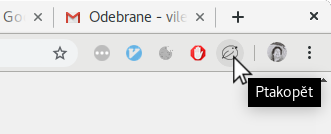
\includegraphics[width=.95\linewidth]{img/ptakopet_old-1/invoke_2}
  \caption{Toolbar icon}
  \label{fig:ptakopet_old-1/invoke_2}
\end{subfigure}%
\begin{subfigure}{.5\textwidth}
  \centering
  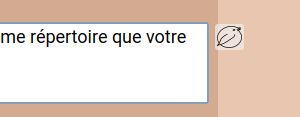
\includegraphics[width=.95\linewidth]{img/ptakopet_old-1/invoke_1}
  \caption{Input element icon}
  \label{fig:ptakopet_old-1/invoke_1}
\end{subfigure}
\caption{Two ways of launching \ptakopet{} old-1}
\label{}
\end{figure}

The \ptakopet{} window could be invoked in multiple ways: by clicking the toolbar button, as shown in \cref{fig:ptakopet_old-1/invoke_1}, by launching it from the context menu (right mouse button) or by clicking an icon, that appeared next to all web page text input elements.

\begin{figure}[ht]
    \centering
    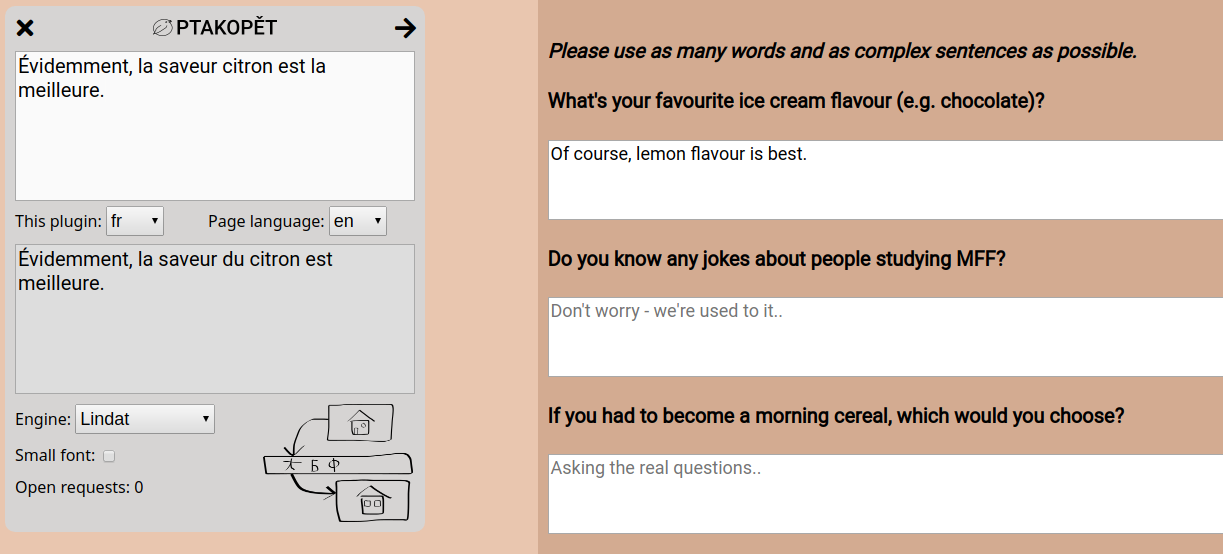
\includegraphics[width=1\textwidth]{img/ptakopet_old-1/ice_cream}
    \caption{\ptakopet{} helps a French-speaking user with filling in an English form}
    \label{fig:ptakopet_old-1/ice_cream}
\end{figure}

In \cref{fig:ptakopet_old-1/ice_cream}, the user selected the first web page input element, hence making it active to \ptakopet{} and wrote a text in their native language (French) to the first \ptakopet{} input. The backward translation removed a definite article for an uncountable noun; otherwise, the sentence matches the original. The English translation of the input sentence then appeared in the target textarea, as expected. Should the user now edit the English text, the translation would appear in the bottom \ptakopet{} textarea. Writing into the top \ptakopet{} input field would overwrite the manual changes, as hinted in the bottom right diagram in the \ptakopet{} window.

\pagebreak 

\subsection{Technical details}

\ptakopet{} old-1 was written entirely with basic HTML, CSS and JS stack with some usage of jQuery. There was no packaging or build system. Part of the codebase dealt with abstraction on top of different browser plugin APIs and the differences between content and background script execution. Most major browsers support the WebExtensions API of W3C, but there are some differences between browsers.

The rest of the code dealt with DOM manipulation and mostly with handling translation requests. Two translation backends were used: Khresmoi \citep{khresmoi} and LINDAT Translation \citep{popel-en-cs}, because of their ease of use and availability. At the time of deployment, LINDAT Translation supported translations between English, French, and Czech, while Khresmoi supported English, French, Czech, German, and Spanish.

Four months after the finished project was demoed, the API which \ptakopet{} used for communication with LINDAT Translation was deprecated and two months after that the Khresmoi translation service shut down. Instead of making necessary fixes, this project was abandoned for a newer version and the plugin was removed from the public listing.

\subsection{Conclusion}

This project was completed and met all criteria regarding quality and functionality, even though the extension was not usable on all websites, which stemmed from the extension architecture.

It was demoed during the Open Days at Charles University Faculty of Mathematics and Physics 2019, although only few visitors tried it. The demo page is not hosted publicly anymore, but source code is available.\footnotehref{https://github.com/zouharvi/ptakopet-old/tree/master/old-1/dod\_ufal}{github.com/zouharvi/ptakopet-old/tree/master/old-1/dod\_ufal} A part of the demo page is visible in \cref{fig:ptakopet_old-1/ice_cream}. The demo included a simple form with random personal questions in a foreign language, which visitors were to fill. The source language in the demo was Czech and, unfortunately, the foreign language was English, so it was hard to demonstrate the issue of outbound translation fully, as most people know English to at least some extent.

A four-page report was submitted.\footnotehref{https://github.com/zouharvi/ptakopet-old/blob/master/old-1/meta/report.pdf}{github.com/zouharvi/ptakopet-old/blob/master/old-1/meta/report.pdf} This first attempt for an outbound translation tool provided us with findings as what to avoid and what to focus on in the next version, \ptakopet{} old-2.

\section{\ptakopet{} old-2}

\subsection{Introduction}

The second version of \ptakopet{} aimed to extend the functionality of the first version, while improving on usability. One of the downsides of the \ptakopet{} old-1 was the disunified behaviour and lack of consistency across different websites. The user interface proved to be too complex to work with and hence we opted for a more traditional approach. The entire application would then be hosted on a separate web page with no interaction with other web pages. This form of serving public machine translation is similar to the one by Google, Microsoft, DeepL and other online services.

In addition to the major change of moving from browser plugin to a standalone web page, we decided to add visual quality estimation cues in the form of word highlighting (from word-level quality estimation models).

\ptakopet{} old-2 was created to meet the requirements of class Semestral Project and has a corresponding specification document.\footnotehref{https://github.com/zouharvi/ptakopet-old/blob/master/old-2/meta/Ptakop\%C4\%9Bt\%20v2\%20-\%20specification.pdf}{github.com/ zouharvi/ ptakopet-old/ blob/ master/ old-2/ meta/ \ptakopet{} v2 - specification.pdf} It was again supervised by Ondřej Bojar.

\subsection{Usage}

There are generally two use cases for the second version: Outbound translation and user translation quality estimation.

\subsubsection*{Outbound translation}

In outbound translation the user tries to translate text to and validate produced translation in a language their are not familiar with.

To perform outbound translation, the user selects the source and target languages from the select box, then writes text in the source language input window (first textarea in \cref{fig:ptakopet_old-2/john_screen}). Problematic words in the source and target text can be seen (more intense colouring means worse quality; purple signifies, that the particular word was not translated) as well as backward translation of the already translated text (third textarea in \cref{fig:ptakopet_old-2/john_screen}).

\begin{figure}[ht]
    \centering
    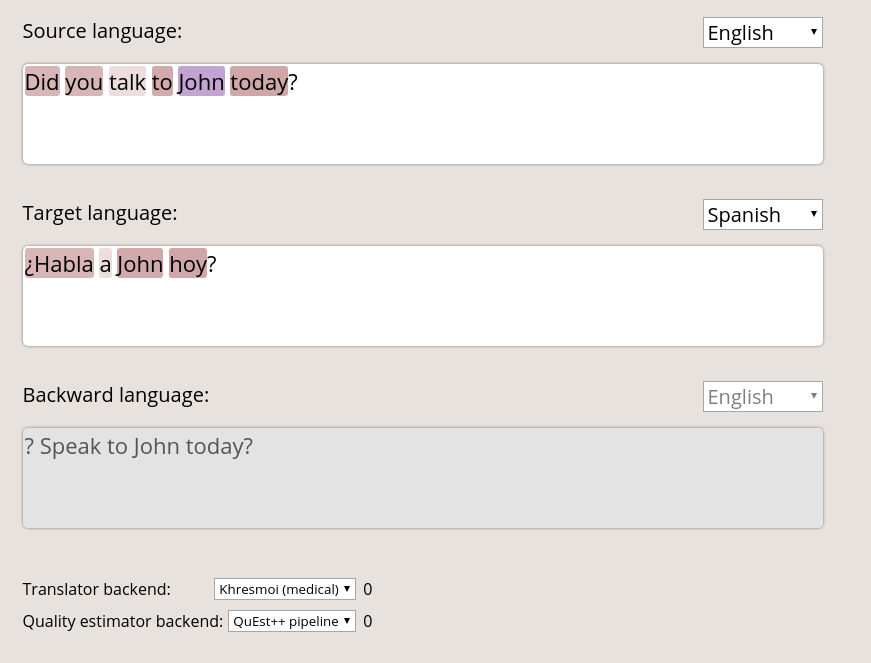
\includegraphics[width=0.85\textwidth]{img/ptakopet_old-2/john_screen}
    \caption{Example usage of \ptakopet{} old-2. The more red the word highlighting, the worse the estimated translation quality. Purple highlighting was used for words, which were not translated.}
    \label{fig:ptakopet_old-2/john_screen}
\end{figure}

\subsubsection*{User translation quality estimation}

The user could then follow up from the previous use case with a more agile workflow and dynamically edit the translated text. They would see the quality estimation of their own translation, as well as backward translation.

In this case the quality estimation is not exactly the same as the task defined by WMT, because the provided translation is not a product of an MT system, but of a human user. With current QE models we do not think that this can be used reliably.

\subsection{Technical details}

The second version was also written in plain HTML, CSS, JS + jQuery (frontend) and Python 3 (backend request handler), but contains many interactions (through system pipes) to other frameworks written in Python 2, Java, Perl and C++. The frontend tech stack is used contrary to modern approaches to web development, but the limited scale of this project and focus on other aspects allowed for it.

The backend ran at servers provided by ÚFAL and responded to requests for either quality estimation or word alignment. The same two translation backends were used: Khresmoi \citep{khresmoi} and LINDAT Translation \citep{popel-en-cs}.

\subsubsection*{Quality Estimation}

There were two quality estimation backends: DeepQuest for English-German and QuEst++ for English-Spanish. 
% The user could select a language pair not compatible with the selected quality estimator, but the result would not be useful, except for their translation quality estimation.

Highlighting parts of texts seems trivial at first, but taking into consideration, that the text must be editable and that the highlighting must work on different zoom levels, browsers and on mobile, it soon becomes complex.
Finally, we opted for a jQuery plugin developed originally by Will Boyd,\footnotehref{https://github.com/lonekorean/highlight-within-textarea}{github.com/lonekorean/highlight-within-textarea} which we forked,\footnotehref{https://github.com/zouharvi/highlight-within-textarea}{github.com/zouharvi/highlight-within-textarea} as some changes to the internal workings of this plugin were necessary.
% (dynamic style attribute instead of based on classes)
We also wanted to highlight words, which were not translated. To do this, we highlighted all words, which were mapped via alignment to a word of the same form. Such an occurrence is displayed in \cref{fig:ptakopet_old-2/john_screen}.

\subsubsection*{Alignment}

Fast align\footnotehref{https://github.com/clab/fast\_align}{github.com/clab/fast\_align} was used for the alignment backend, as it was recommended in the QuEst++ documentation. Word alignment was necessary for the highlighting itself as well as for QuEst++.

\subsection{Issues}

We later found that we used Fast align incorrectly, applying the unsupervised word-alignment method only to the single input sentence pair given. Since the model lacks any lexical knowledge, it thus essentially provided a simple diagonal alignment most of the time.

Because of missing Access-Control-Allow-Origin header on the Khresmoi translator backend, a proxy was added. This was unavoidable but a wrong decision since it is considered unsafe and software such as Avast would notify the users.

At the time of the deployment, the web hosting server had a valid SSL certificate but made requests to unsafe servers, so it had to be served over HTTP.

Another issue was the lack of a clear indication of supported language pairs. \ptakopet{} allowed users to use a quality estimation model even for language pairs that the model did not support.

Setting up the server was also a difficult task, as proper replicable setup scripts were not written.

\subsection{Conclusion}

While \ptakopet{} old-2 passed as a semestral project, there were many ideas on how to improve the experience and project quality. In \ptakopet{} old-2 only English-Spanish and English-German language pairs were supported by QuEst++ and DeepQuest respectively. Especially DeepQuest could be used with more language pairs if relevant data were provided. DeepQuest also reported only binary values \texttt{OK} or \texttt{BAD} at that time, but continuous confidence values from 0 to 1 existed inside. Extracting them would have provided more information to the user.

During development, the whole project accumulated significant technical debt. This was due to decisions such as writing in JavaScript without a framework, not having more structured backend and missing setup scripts.

Both technical and user documentation\footnotehref{https://ptakopet.vilda.net/docs/old-2}{ptakopet.vilda.net/docs/old-2} was written on this version.

\newpage

\section{Industry} \label{sec:related_industry}

As far as we observed, modern outbound translation workflow is condensed to roundtrip translation done manually by users (switching the language direction and copy-pasting the translated text).

Quality estimation is used in translation companies mostly to minimize post-editing costs. Despite that, QE cues are missing in most of the mainstream public translation services, such as Google Translate\footnotehref{https://translate.google.com/}{translate.google.com} (provides alternatives to words and shows their usage frequencies), Microsoft Bing Translator\footnotehref{https://www.bing.com/translator}{bing.com/translator} or DeepL\footnotehref{https://www.deepl.com/en/translator}{deepl.com/en/translator} (provides alternatives to phrases).

\subsubsection{Memsource}

The company Memsource, which specializes in cloud-based translation environment with tools like translation memory and terminology management, is also deploying quality estimation models, to minimize post-editing cost. For example, if a machine-translated sentence receives a full score, then there is no need to pay professional human translators to verify the translation. Even though they are developing their models in-house and closed-source, they disclosed some details in one of their blog posts.\footnotehref{https://www.memsource.com/blog/2018/10/01/machine-translation-quality-estimation-memsources-latest-ai-powered-feature/}{memsource.com/blog/2018/10/01/machine-translation-quality-estimation-memsources-latest-ai-powered-feature/}

Notable is their way of presenting the quality estimation data. Instead of displaying the percentage score in any form (e.g. highlighting), they approach this as a classification problem with the classes: $100\%$: probably perfect translation, $95\%$: possibly requires minor post-editing, $85\%$: will require post-editing, no score: needs to be manually checked. They focus on the phrase-level and sentence-level quality estimation.

\subsubsection{Unbabel}

The company Unbabel, which delivers machine translation solutions, is also developing\footnotehref{https://unbabel.com/blog/unbabel-translation-quality-systems/}{unbabel.com/blog/unbabel-translation-quality-systems/} a QE pipeline. As opposed to Memsource, most of their QE research is public, such as \cite{martins-unbabel:2016} and \cite{openkiwi}. They also make use of both word-level and phrase-level quality estimation. One of their components, OpenKiwi, is also part of \ptakopet{} and is described in \cref{subsec:openkiwi}.
\chapter{Final \ptakopet{}} \label{chp:usage}

The final version of \ptakopet{} is publicly accessible from \href{https://ptakopet.vilda.net}{ptakopet.vilda.net}. The goals of this version were to improve the overall user experience, make the system more modular, scalable and robust and also to make it ready for experiments on human annotators.

\section{Overview}

\ptakopet{} helps users with outbound translation. The full layout is displayed in \cref{fig:usage-1}. It is composed of four blocks (modules): input, translation, backward translation, paraphrases. Source and target languages can be selected in the drop-down menus at the top of the first two modules. After writing text in the first textarea, it is translated to the second textarea (also editable), then backward translation, quality estimation and paraphrases are generated.

\begin{figure}[ht]
  \centering
  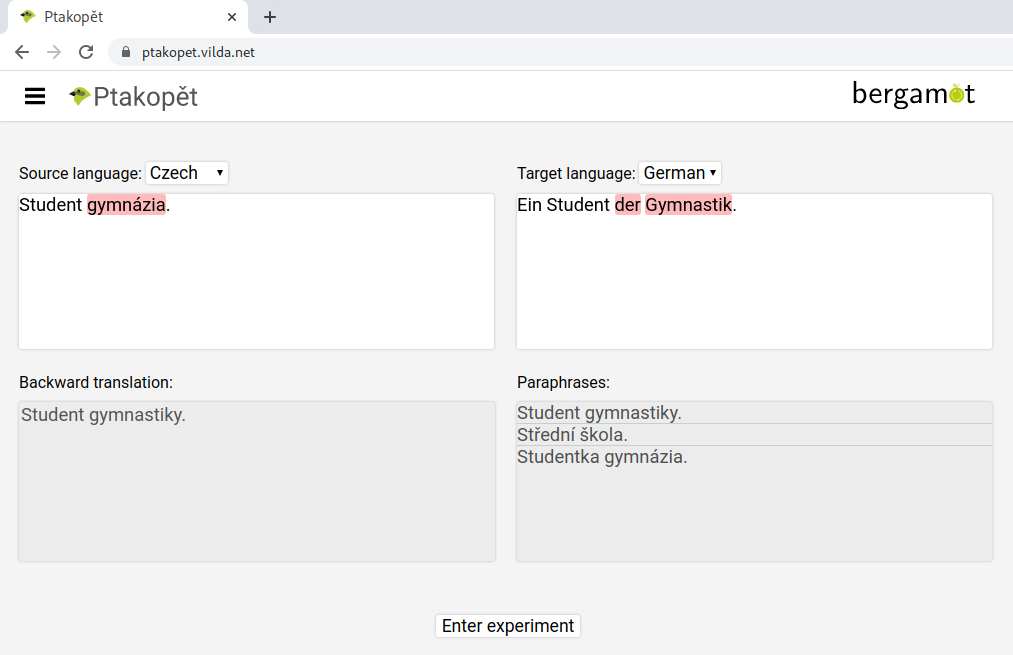
\includegraphics[width=\textwidth]{img/usage/usage-1.png}
  \caption{\label{fig:usage-1} \ptakopet{} is used to translate a simple Czech noun phrase to German. QE highlights parts of both source and target, that were translated incorrectly.}
\end{figure}

In \cref{fig:usage-1} it is seen, that the source was mistranslated by the red highlighting (on both source and target), but also by the backward translation. Paraphrases (or source variations) are displayed in the second to last block. In the case of simple noun phrases, they are irrelevant, but they are useful for more complex inputs, as shown in \cref{fig:usage-2}. In those cases, the user might want to reformulate (mostly simplify) specific parts of their input, so that the MT system can produce a better translation. 

Unfortunately, we found the quality estimation not to be reliable enough. It usually works only with concise sentences or simple noun phrases. This can be seen when comparing the highlighting in \cref{fig:usage-1} and \cref{fig:usage-2}.

The translation can be then also edited. A common error of MT systems is that they try to translate named entities. This is easy to recognize even in languages the user is not proficient in. They may then choose to fix this error in the translation textarea and check that all went well in the backward translation block. Typing anything in the source textarea would then rewrite these manual changes.

The backend for each service can be selected in the settings burger menu, hidden behind the burger icon in the top left corner in \cref{fig:usage-1}. The expanded settings menu is shown in \cref{fig:usage-settings} in the last block. Changing any language or backend selection causes a cascade so that relevant information is recomputed and showed. Pending requests to a specific backend are signalized by a loading indicator next to every module block.

\begin{figure}[ht]
  \centering
  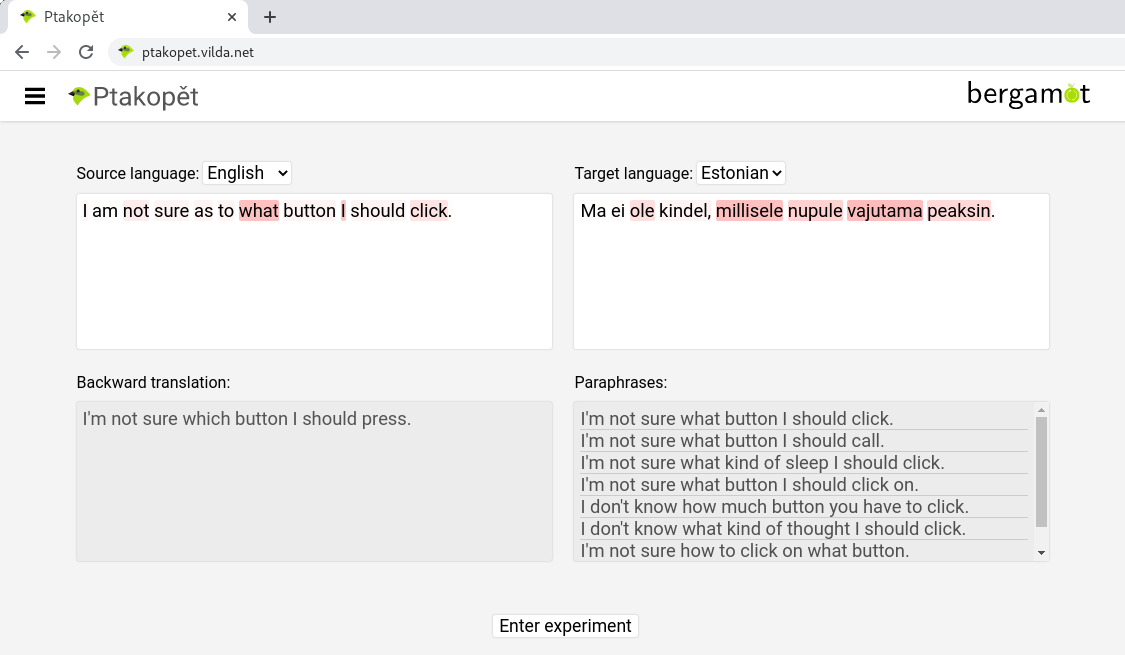
\includegraphics[width=\textwidth]{img/usage/usage-2.png}
  \caption{\label{fig:usage-2} \ptakopet{} is used to translate a complex English sentence to Estonian. User may opt to reformulate the input according to the paraphrases suggestions.}
\end{figure}

\begin{figure}[ht]
  \centering
  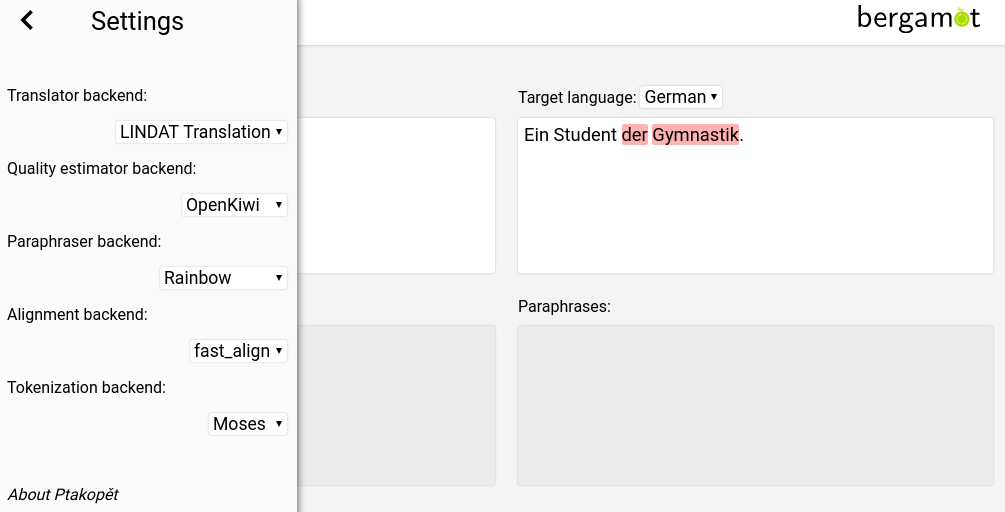
\includegraphics[width=\textwidth]{img/usage/usage-settings.png}
  \caption{\label{fig:usage-settings} Expanded settings burger menu in \ptakopet{}, which allows the users to change service backends.}
\end{figure}

\section{Settings overview}
\label{sec:usage-settings}

Backend settings are freely accessible, even though we do not expect most users to interact with them. Some particular settings are not intended to be used for outbound translation but are included either as placeholders or for debugging or presentation purposes. In this section, we aim to give a brief overview of their respective roles and origins. Backends, which were not created or setup by the author of this thesis, are explicitly mentioned.

An exclamation mark is shown next to the specific module in case the selected backend is incompatible with a given language pair. This warning is seen in \cref{fig:usage-mobile}.

\subsection*{Translator}

The main translator backend is \backendname{LINDAT Translation} \citep{popel-en-cs}, which provides translations between Czech, English, French and German. \backendname{Strong EN-CS} is just a shadow copy of this backend. Due to a collaboration with Tartu on the Bergamot project, we also added English$\leftrightarrow$Estonian backend \backendname{Neurotõlge}\footnotehref{https://neurotolge.ee/}{neurotolge.ee} and \backendname{Avg EN-ET}. For future experiments, we also added \backendname{Weak EN-CS} and \backendname{Strong EN-CS} for English$\leftrightarrow$Czech translation at various quality. There are also two placeholder backends, which evaluate client-side. \backendname{Identity} only copies the input and \backendname{None/Manual} does nothing so that the user can input their own texts without being interrupted. All of the non-local backends are not part of the work on this thesis.

\subsection*{Quality Estimation}

Our instances of \backendname{OpenKiwi} and \backendname{DeepQuest} backends support Czech$\rightarrow$German and English$\rightarrow$German quality estimation. The running instance of \backendname{QuEst++} supports English$\rightarrow$Czech quality estimation but is of very low quality. Collaborators from the Bergamot project who specialize in quality estimation provided two backends \backendname{Sheffield EN-ET} and \backendname{Sheffield EN-CS}. For presentation purposes, the QE values can be inputted manually by selecting the \backendname{Manual} backend. It can also be set to \backendname{Random}, which assigns each target word a random value between 0 and 1. This fake backend is good for analyzing alignment because one can then easily see what the words map to. The highlighting can be turned off by selecting \backendname{None}.

\subsection*{Paraphraser}

The first paraphraser is \backendname{LINDAT Mock}, which relies on round-trip translation with LINDAT Translation. It is extremely unoptimized and is there only for testing purposes. The second paraphraser backend, \backendname{Rainbow}, works on a similar principle but is more elaborate and faster. This backend is a transformer-based and is the work of Matúš Žilinec.\footnotehref{https://github.com/mzilinec/paraphrase-server}{github.com/mzilinec/paraphrase-server} The paraphraser module can also be turned off by selecting \backendname{None} as the paraphraser backend.

\subsection*{Alignment}

Alignment requests for most languages are by default relayed to \backendname{fast\_align Ubuntu} on server-side. There also exists a special backend \backendname{fast\_align Michal} which was setup by a colleague Michal Novák for future experiments with \ptakopet{} on English-Estonian and English-Czech language pairs. The alignment can also be evaluated locally by \backendname{Diagonal} placeholder backends, which for sentences of $M$ and $N$ tokens generates alignment $\{(i, j): 0 \le i \le M, 0 \le j \le N\}$. The \backendname{None} turns off the alignment altogether.

\subsection*{Tokenization}

The \backendname{Moses} tokenizer is the main tokenization backend and is very robust. There are two alternatives, which evaluate client-side. The first one, \backendname{Spaces}, is just splitting by single spaces, while the second one, \backendname{Local}, uses a more complex tokenization scheme.

\section{Miscellaneous}

\subsection*{Omnibox OpenSearch}
Google services and most notably Google Translate use omnibox OpenSearch to improve the user experience. This was also implemented in \ptakopet{}, so instead of having to go to the web page and then start typing the source text, it can be typed in the address bar after pressing the \texttt{TAB} key. The web page is then loaded and the input pasted in the input textarea.

This makes it more convenient for using \ptakopet{} to quickly translate pieces of texts. An example omnibox input and the result is shown in \cref{fig:usage-omnibox}.

\begin{figure}[ht]
  \centering
  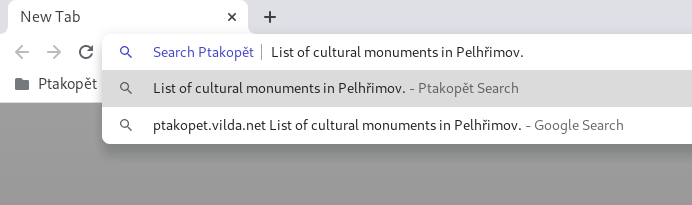
\includegraphics[width=\textwidth]{img/usage/omnibox-opensearch-1.png}
  \text{}\vspace{0.5cm}
  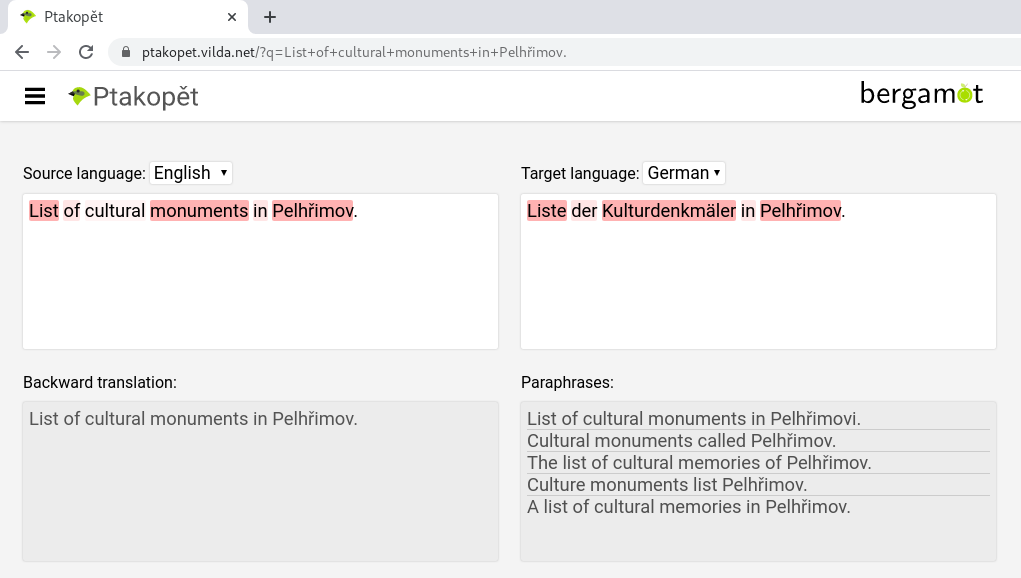
\includegraphics[width=\textwidth]{img/usage/omnibox-opensearch-2.png}
  \caption{\label{fig:usage-omnibox} Example usage of omnibox OpenSearch input. The text appears in the main input textarea once the user hits \texttt{ENTER}. The default language and backends settings are used.}
\end{figure}

\pagebreak

\subsection*{URL parameters}

\ptakopet{} also supports other URL GET parameters:
\begin{itemize}
    \item \texttt{userID} logs the user to the experiment by the supplied userID value. The experiment is discussed in \cref{sec:experiment_def} and \cref{chp:experiment}.
    \item \texttt{q} pastes the text query into the input box. This is to support the omnibox OpenSeach functionality.
    \item \texttt{p} sets a given settings profile to other than \texttt{default}, e.g. \texttt{pilot}, \texttt{edin}, \texttt{csen} or \texttt{sao}. This is helpful when one wishes to provide a quick link with all settings prepared. These exact settings profiles were used for different presentation purposes.
    \item \texttt{source} sends this extra value to the start log.
    \item \texttt{test} used for testing, described in \cref{subsubsec:implementation_testing}.
\end{itemize}

The redirect URL for profile \texttt{pilot} with the user \texttt{testuser} and source information \texttt{online-ad} can then look like:

\texttt{ptakopet.vilda.net/?p=pilot\&userID=testuser\&source=online-ad}

\subsection*{Error masking in backtranslation} \label{sec:error_masking}

When using the same data for both forward and backward MT, an error can be introduced in forward translation but removed in the backward translation. After experimenting with \ptakopet{} we found several examples described in \cref{fig:error_masking_example}. All can be tested in the live system using the \backendname{LINDAT Translation} backend.

\begin{figure}[ht]
    \begin{align*}
        \text{svírá úhel} \hspace{1cm} &\xrightarrow{\text{de}} &\text{Er schließt den Winkel.} \hspace{1cm} &\xrightarrow{\text{cs}} &\text{Zavírá úhel.} \\
        \text{svírá úhel} \hspace{1cm} &\xrightarrow{\text{fr}} &\text{Sait l'angle} \hspace{1cm}  &\xrightarrow{\text{cs}} &\text{Zná úhel} \\
        \text{svírá úhel} \hspace{1cm} &\xrightarrow{\text{en}} &\text{grips the angle} \hspace{1cm}  &\xrightarrow{\text{cs}} &\text{svírá úhel} \\
    \end{align*}
    \caption{\label{fig:error_masking_example} Example of error masking in backward translation in English MT compared to German and French MT in which the error is revealed.}
\end{figure}

The German and French MT in \cref{fig:error_masking_example} introduced an error in forward translation, but the backward translation was accurate and thus, the user could recognize this and reformulate the input. However, in the case of the English machine translation, an error is still introduced in the forward translation but the backward translation removes this error. The backward translation could, in fact, be accurate and this masking could be a result of sense ambiguity of the word ``svírat''. Nevertheless, the user could then get a false sense of a correct translation, which is undesirable.


\subsection*{Platforms}

\begin{figure}[ht]
  \centering
  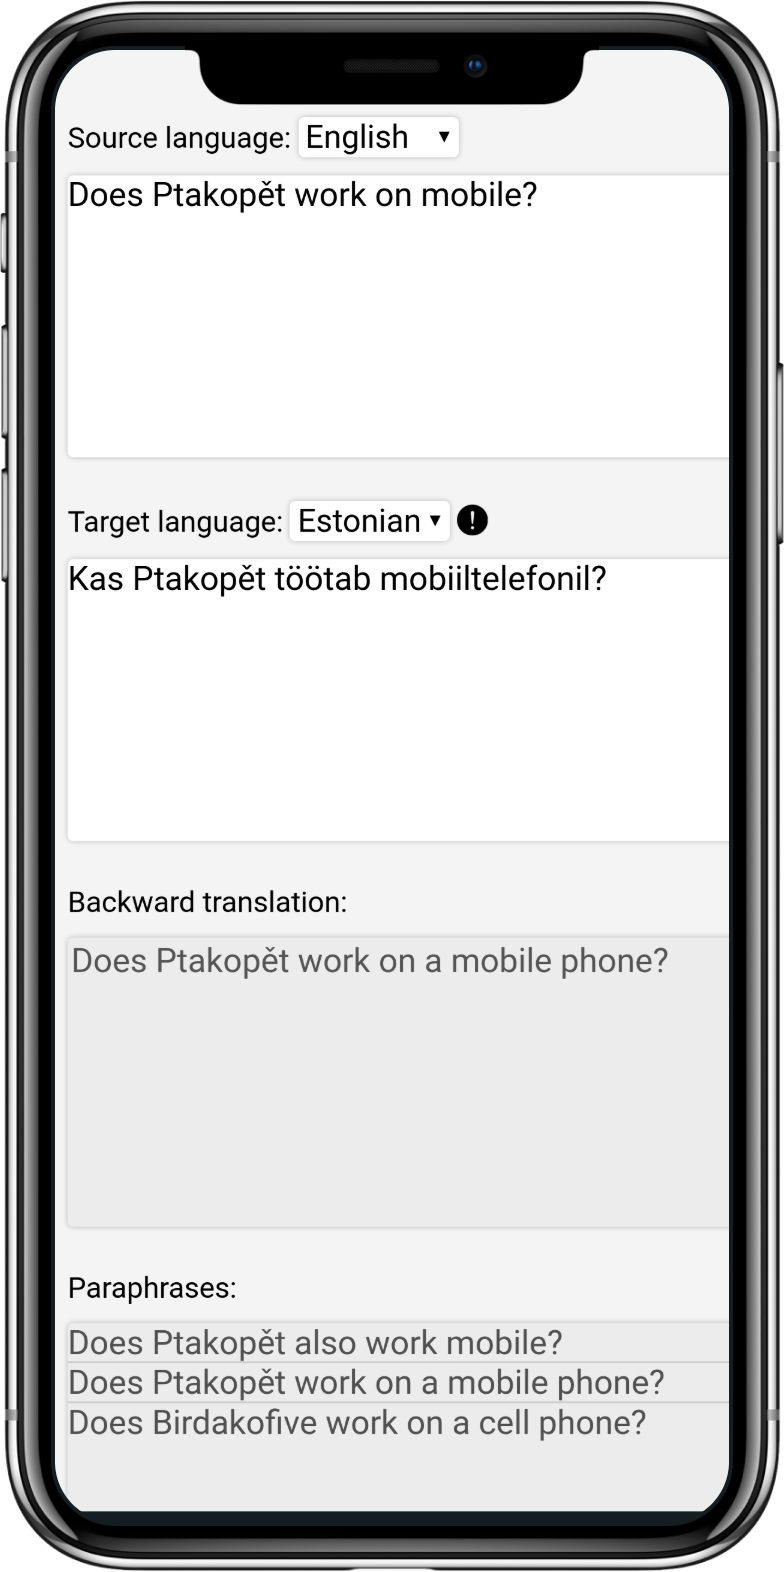
\includegraphics[width=0.45\textwidth]{img/usage/usage-mobile-mockup.png}
  \caption{\label{fig:usage-mobile} Mockup of \ptakopet{} in single column layout on phone.}
\end{figure}
% https://dimmy.club/phones/iphone-x

\ptakopet{} was tested to run properly on Edge 80, Chrome 83, Firefox 75 and Opera 66.

We wanted \ptakopet{} to be accessible from as many devices as possible and not just desktops. The frontend was designed to adapt to almost any screen size, most notably mobile. The layout is then changed to a single column, as shown in \cref{fig:usage-mobile}.

We found \ptakopet{} to be very usable on mobile. The only issue was that occasionally deleting of already written text could not be done by holding the backspace key. This is due to the highlighter dependency. \ptakopet{} was also tested to work without any issues on very computationally limited device, namely Samsung Smart TV with Tizen OS.
\chapter{Implementation} \label{chp:implementation}

The whole project is split into two git repositories hosted at GitHub. The first repository\footnotehref{https://github.com/zouharvi/ptakopet}{github.com/zouharvi/ptakopet} contains the code for frontend, experiment data as well as some miscellaneous files regarding the whole project. The second one\footnotehref{https://github.com/zouharvi/ptakopet-server}{github.com/zouharvi/ptakopet-server} is focused strictly on the server, which is not the main focus of this thesis but is also described for completeness.

In this chapter we first describe the frontend, then the experiment architecture from a technical perspective (the experiment itself is the focus of \cref{chp:experiment}) and then the backend. See documentation in \cref{chp:development_doc} which describes all the implementation details as well as guides on how to build and setup the whole project.

\section{Frontend}
\label{sec:implementation:frontend_structure}

The web frontend is written in TypeScript because of the great scalability properties. DOM manipulation is done mostly with jQuery and the output is packed into one JavaScript file using Webpack. Packages are managed with npm (usually contained in the NodeJS package).

\begin{figure}[ht]
    \centering
    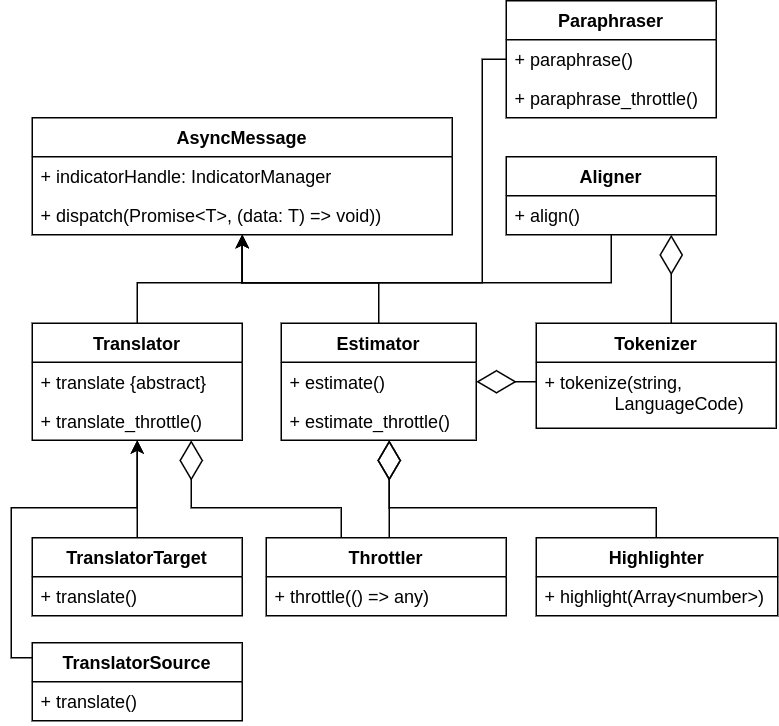
\includegraphics[width=\textwidth]{img/implementation/frontend.png}
    \caption{Object diagram of main component of the \ptakopet{} frontend}
    \label{fig:frontend_class}
\end{figure}

The diagram in \cref{fig:frontend_class} shows the overall object structure of the most important objects. These objects are: \texttt{AsyncMessage}, \texttt{Translator} (and its derivatives), \texttt{Estimator}, \texttt{Aligner}, \texttt{Paraphraser}, \texttt{Tokenizer}, \texttt{Highlighter} and \texttt{Throttler}. 

The task of \texttt{TranslatorSource} (and similarly for \texttt{TranslatorTarget}) is to translate the source sentence. Then \texttt{Estimator} has to assign word-level quality estimation scores for each target token. Finally, a word-level alignment must be computed in \texttt{Aligner}. At the end, the QE is rendered using \texttt{Highlighter}. Parallel to that, \texttt{Paraphraser} produces paraphrases for the source input and displays them.

Each of these computations could take place in the browser\footnote{This one of the goals of the Bergamot project. \href{https://browser.mt/}{browser.mt}} (\ptakopet{} includes some such mock-up solutions, see \cref{sec:usage-settings}), but the standard procedure is to relay the translation, estimation, paraphrase, alignment and tokenization requests to some server.

\subsubsection*{AsyncMessage}

Since there can be multiple such requests of one type in one second, it is possible to get into a race condition. This is what happened in the \ptakopet{}-old projects and vastly worsened the user experience.

Sometimes a translation request, which was sent later than another one, would finish sooner. The new content would be presented, but then the old request would then finish and outdated content would be shown. This is highly undesirable and it is the reason why most of the messaging objects (\texttt{Translator}, \texttt{Estimator}, \texttt{Paraphraser}) make use of \texttt{AsyncMessage}. This class assigns a serial number to each request and drops delayed incoming responses. By keeping track of active requests, \texttt{AsyncMessage} derivatives can easily display an indicator to the user, signalizing whether it is still waiting for a response or not.

The other messaging components, \texttt{Tokenizer} and \texttt{Aligner}, do not have any callback, which results in any content manipulation (they are almost pure functions) that are invoked solely using \texttt{async/await}.

\subsubsection*{Backends} \label{subsubsec:impl:backend}

Each of the main messaging components contains a list of backends so that they can be easily interchanged and tested. These ``backends'' are not to be confused with the server backend, described in \cref{sec:server-backend}. A backend in this context is just an object, which contains a list of supported language pairs, a name and a function, which for some input returns a promise of the relevant output. A definition of a quality estimation \backendname{Random} backend is available in \cref{subsubsec:dev_doc:backend}.

\pagebreak
\subsubsection{Miscellaneous objects}

Apart from the main object distinguished in the diagram in \cref{fig:frontend_class}, there are many others. We list a brief overview of their functionality.

\begin{itemize}
    \item \texttt{Throttler} - a simple tool for handling throttling. The input event (on the source input field) fires up every time the user types in a character. It is undesirable to send a translation request after every keystroke, so the throttler sends only the last request and only if no input event happened for some duration. This is achieved by \texttt{window.setTimeout} which restarted every time input event happens.
    \item \texttt{Utils}, \texttt{TextUtils} - various helper functions, such as generating a set of all possible pairs from a set, language code database, parameter parsing, random string generation.
    \item \texttt{Settings} - globally accessible and simply stores the currently selected backend and language options.
    \item \texttt{SettingsSelector} - backend and language selection in the DOM.
    \item \texttt{SettingsProfiles} - defines common setting setups, which can be later applied (e.g. \texttt{default} and \texttt{pilot})
    \item \texttt{Highlighter} - quality estimation DOM element highlighting
    \item \texttt{Tester} - contains functions used for testing
\end{itemize}

\begin{figure}[ht]
    \centering
    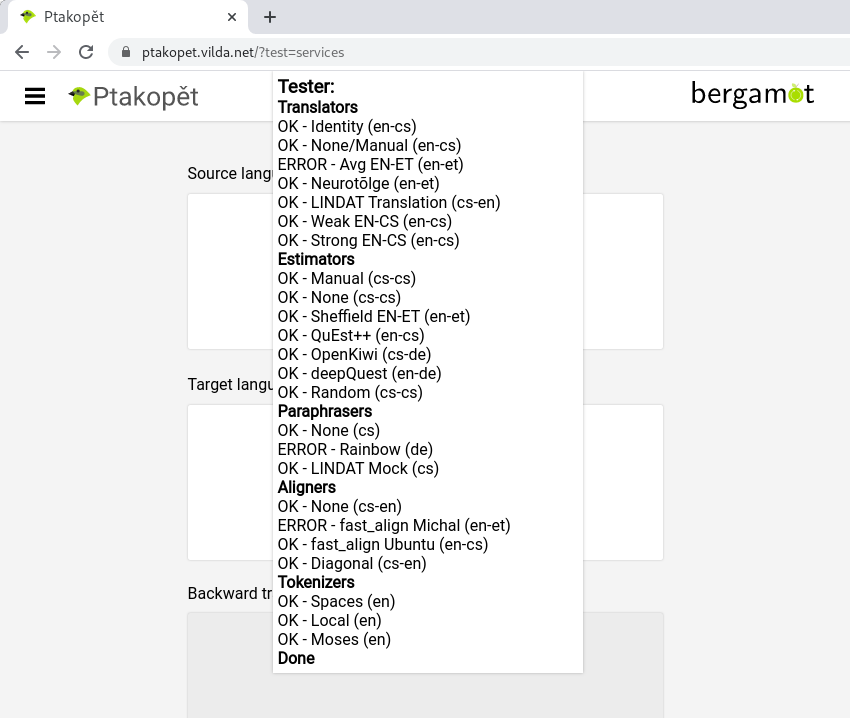
\includegraphics[width=\textwidth]{img/implementation/test_services.png}
    \caption{Results of testing of all \ptakopet{} backends. Three backends were down at the moment.}
    \label{fig:test_services}
\end{figure}

\subsubsection{Testing} \label{subsubsec:implementation_testing}

The \texttt{Tester} class contains two functions. The first one, \texttt{workload}, simulates the user's workflow by changing the source input field in some fixed interval. This was used for debugging memory leaks, such as the one which was present in the pilot study (\cref{subsubsec:experiment_leak}). It can be invoked by adding the \texttt{test=workload} URL GET parameter.

The other function is used for testing the availability of backends. Since \ptakopet{} encompasses many backends it is necessary to monitor their status. To get a summary of their availability add the \texttt{test=services} URL GET parameter. A white window will then appear at the top of the screen. The result is visible in \cref{fig:test_services}. This function sends requests to all available backends (even local ones) with a prepared text input and language settings. Usually the backend status (up or down) is manifested on a single call, so checking text and language variations is not necessary.


\subsubsection{Highlighting} 

Given a QE score from $0$ to $1$ the color is computed as in \cref{equation:implementation_color}. It is substracted from one, because QE of $1$ correspond to high confidence and we want to highlight bad scores. It is also scaled down by $\frac{1}{3}$ for the highlighting to not be too disruptive in the user interface. Technical details of highlighting are described in \cref{subsubsec:dev_doc:highlighting}.

\begin{equation}
        \text{color}(qe) = \text{RGBA}\big(1, 0, 0, \frac{1-qe}{3}\big)
    \label{equation:implementation_color}
\end{equation}

\subsubsection{Source complexity} \label{subsubsec:impl:source_complexity}

After the quality estimation and alignment is computed, every source word receives a possibly empty set of QE scores. This is because the alignment may map the source word to zero or more target words. Different aggregating functions can be chosen to get a single number, for example \textit{maximum}, \textit{minimum}, \textit{average} or \textit{weighted average (by position)}. Furthermore the default QE score has to be assigned to unaligned tokens. We found it reasonable to use the \textit{average} aggregating function as to consider all the provided scores. The score for unaligned tokens was set to $0.9$ to only slightly hint that something may be wrong.

\pagebreak
\section{Experiment definition} \label{sec:experiment_def}

An experiment can be defined in a single JSON file. The format, details and relevant tools used for generating experiment materials are described in detail in \cref{sec:dev_doc:experiment_def}.

In the experiment definition we need to specify the number of users, their user IDs and the queues. In this context we use the term ``baked queues'' for every user which is just pre-generated random sequence of stimuli and their configurations. This way it is decided prior to the experiment what stimuli configurations and in what order will a given users encounter them. Baked queues are described more in detail in \cref{subsec:experiment:technical_details}.

A stimuli is just a string containing a HTML code which gets pasted into the webpage. This is flexible enough to allow for both images and texts with highlights. Every stimuli can be also presented with a different configuration, such as a specific backend and set of modules enabled.


\section{Server backend}
\label{sec:server-backend}

The server backend's purpose is to make some of the MT related services (quality estimation, alignment, tokenization) available to the frontend. It is necessary, as most of these services are not publicly deployed, but is not the main focus of the \ptakopet{} project, nor of this thesis. Even though it was created to be portable in theory, it is not expected to be run on any other server than ours. It is written in Python~3.

To run the server (on \texttt{0.0.0.0:80}), launch the \texttt{server/run.sh} script. A common practice is to connect to a remote machine via SSH and launch the server. For that, there is a script \texttt{server/run\_nohup.sh}, which disregards kill signals on user logout.

\begin{figure}[ht]
    \centering
    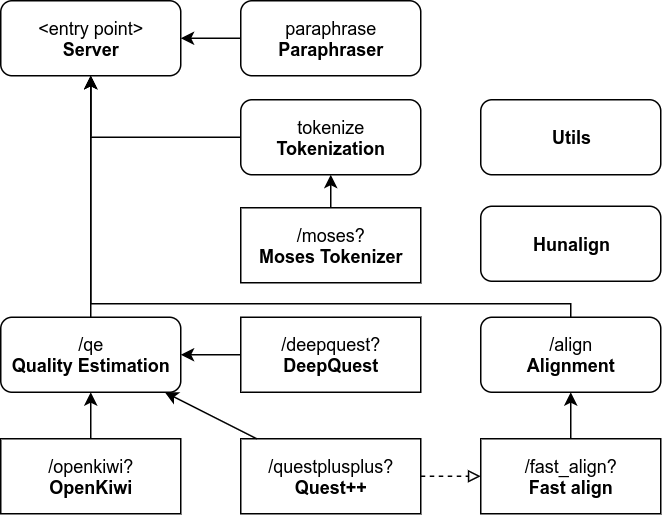
\includegraphics[width=0.8\textwidth]{img/implementation/backend.png}
    \caption{Object diagram of main components of the \ptakopet{} backend}
    \label{fig:backend_class}
\end{figure}

\subsection{Architecture and API}

The overall backend object architecture is shown in \cref{fig:backend_class}. The dashed line from QuEst++ to Fast align means that QuEst++ uses this alignment tool also as part of its pipeline. Both GET and POST methods are accepted. The server offers the following API calls. In \cref{lst:backend_examples_1} and \cref{lst:backend_examples_2}, we show example requests together with their responses. The sentence aligner Hunalign is not accessible publicly and is used only for internal purposes.


\begin{itemize}
    \item \texttt{qe/[openkiwi, deepquest, questplusplus]/?} - for word-level QE. \\
    Requires: \texttt{sourceLang} \texttt{targetLang}, \texttt{sourceText} and \texttt{targetText}.
    
    \item \texttt{align/[fast\_align]/?} - word alignment. \\
    Requires: \texttt{sourceLang} \texttt{targetLang}, \texttt{sourceText} and \texttt{targetText}.
    
    \item \texttt{tokenize/[moses]/?} - sentence tokenization. \\
    Requires: \texttt{text} and \texttt{lang}.
    
    \item \texttt{paraphrase/[mock]/?} - paraphrasing. \\
    Requires: \texttt{text} and \texttt{lang}.
\end{itemize}


\begin{lstlisting}[caption={Three examples of \ptakopet{} backend quality estimation, tokenization and alignment requests and responses}, label={lst:backend_examples_1}, escapeinside={\%*}{*)}, stringstyle=\ttfamily, showstringspaces=false]
qe/deepquest
    ?sourceLang=cs
    &targetLang=de
    &sourceText=%*Student gymnázia.*)
    &targetText=Ein Student der Gymnastik.
    
-> {"status": "OK", 
    "qe": [0.8, 0.5, 0.2, 0.5, 1.0]}

tokenize/moses
    ?text=(z.B. Tomaten, Karotten usw.)
    &lang=de
    
-> {"status": "OK",
    "tokenization": ["(", "z.B.", "Tomaten",
                     ",", "Karotten", "usw.", ")"]}
               
align/fast_align
    ?sourceLang=en
    &targetLang=de
    &sourceText=Click the mouse button.
    &targetText=Klicken Sie mit der Maustaste.
    
-> {"status": "OK",
    "alignment": "0-0 0-1 2-2 1-3 3-4 4-5"}
\end{lstlisting}
               
\begin{lstlisting}[caption={An example of \ptakopet{} backend paraphrase request and response}, label={lst:backend_examples_2}, escapeinside={\%*}{*)}, stringstyle=\ttfamily, showstringspaces=false]
paraphrase/mock
    ?lang=cs
    &text=%*Jsem student posledního ročníku gymnázia.*)
    
-> {"status": "OK",
    "de": %*"Poslední rok studuji gymnastiku.",*)
    "fr": %*"Jsem v posledním ročníku střední školy.",*)
    "ru": %*"Jsem ve čtvrťáku na gymnáziu.",*)
    "en": %*"Jsem ve čtvrťáku na gymnáziu."*)}
\end{lstlisting}


\subsection{Data and trained models}

\subsubsection{Word alignment}

Fast align is the only alignment model we deployed. It simply requires a bilingual sentence aligned corpus. We add the incoming language pairs to the data and run Fast align. For the corpora, we make use of Ubuntu localization files.\footnotehref{http://opus.nlpl.eu/Ubuntu-v14.10.php}{opus.nlpl.eu/Ubuntu-v14.10.php} We chose the IT domain, because data for the QE models are only in this domain. The server is distributed with the following language pairs: \texttt{cs-de}, \texttt{cs-en}, \texttt{cs-fr}, \texttt{en-de}, \texttt{en-es}, \texttt{en-et} and \texttt{en-fr}.

\subsubsection{Quality estimation}

The original feature extractor system in QuEst++ supports English$\rightarrow$Spanish quality estimation. We experimented with feeding it English$\rightarrow$Czech quality estimation data and expected that the ML part would disregard noisy or low information features caused by feeding the feature extractor unsupported language. We found that the performance regressed so considerably that we did not experiment further and focused on other QE systems.

Both DeepQuest (bRNN) and OpenKiwi (Predictor-Estimator) were trained on WMT 2017 English-German Word Level Quality Estimation dataset in the IT domain \citep{WMT17}. These trained models are downloaded automatically when running the backend install script. 
OpenKiwi, in general, proved to be faster, more robust and easier to use than DeepQuest. Because of this, the experiment was conducted with OpenKiwi quality estimation backend.

\subsubsection{Czech-German Quality Estimation Dataset} \label{subsec:cs_de_wmt}

For the experiment, we also needed to train a Czech$\rightarrow$German QE model. Since relevant Czech$\rightarrow$German training data for QE were not available, we synthesized them from English$\rightarrow$German data. We processed the WMT17 English-German data to obtain Czech$\rightarrow$German data by translating the source language sentences using LINDAT Translation \cite{popel-en-cs} from English to Czech. Given triplets (English, German, QE), we thus create triplets of (Czech, German, QE). An example of this can be seen in \cref{fig:tripel_qe_example}.

\begin{figure*}[ht]
    \centering
    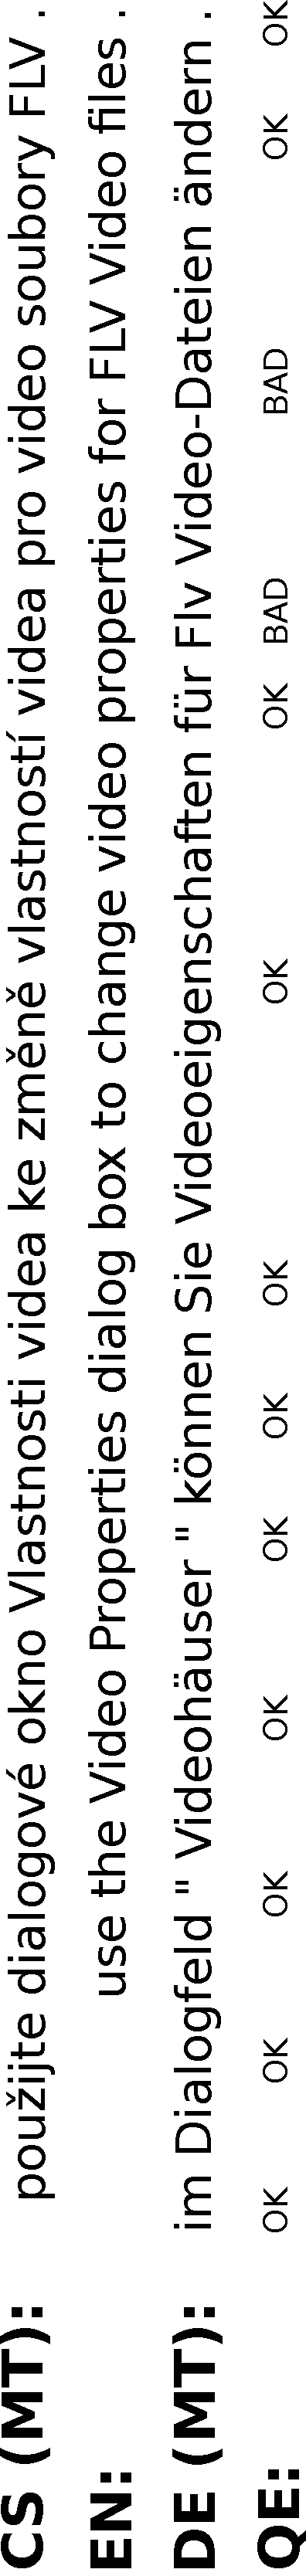
\includegraphics[height=\textwidth, angle=-90]{img/implementation/qe_example_pdfa1a.pdf}
    \caption{\label{fig:tripel_qe_example} Quality estimation tags for tokens and gaps on German sentence translated from English (from WMT19 quality estimation shared task) together with synthetic Czech source (translated from English). MT systems are independent.}
\end{figure*}

To make sure the data did not lose quality, we performed the following experiment: We manually annotated 30 Czech-German and 20 English-German sentences for word-level quality estimation, in the same format as the original English-German dataset, i.e., labeling German words with OK/BAD labels given the source sentence. The original English-German annotation served as the golden standard. Our annotation for English-German was created independently of it and it served as a benchmark for our agreement with the original. 

\begin{table}[ht]
    \centering
    \begin{tabular}{| l l |}
        \hline
        \multicolumn{2}{|c|}{All}\\
        \hline
        TP=74.57\%& FP=2.68\%\\
        FN=12.98\%& TN=9.76\%\\
        \hline
        \multicolumn{2}{|c|}{Czech$\rightarrow$German}\\
        \hline
        TP=77.58\%& FP=3.68\%\\
        FN=11.03\%& TN=7.71\%\\
        \hline
        \multicolumn{2}{|c|}{English$\rightarrow$German}\\
        \hline
        TP=69.81\%& FP=1.11\%\\
        FN=16.07\%& TN=13.02\%\\
        \hline
    \end{tabular}
    \caption{\label{tab:manual_qe_annotation}Confusion matrix for word-level quality estimation annotations of Czech-German and English-German.}
\end{table}

\cref{tab:manual_qe_annotation} shows the confusion matrices of our annotations compared to the golden standard. The distributions for both language pairs are similar. The sample is very small and the sets of underlying sentences (20 English and 30 Czech) had to be different because the annotation was carried out by a single person, but the results nevertheless indicate that this transfer of QE data by machine-translating the source is viable. The similarity of confusion scores can mean one of the following. Either the German sentence itself was representative enough for the annotator to produce classes with similar distributions, or that both the English and the Czech sentences provided the same level information. In both cases, the pairs (EN, DE) and (CS, DE) seem equally usable, which means that we should be able to train a similarly good quality estimation model based on the synthetic Czech source.
\chapter{Experiment}
\label{chp:experiment}

To test the usability of the \ptakopet{} tool proposed in this thesis, we designed an experiment. This experiment aimed to classify and describe strategies users take when tasked to do outbound translation, as well as the final quality of the produced texts. It was the main focus of one of the papers connected to this thesis \citep{zouhar:ptakopet}.

\section{Setup}

The experiment was carried out remotely, in two phases. In the first phase, annotators were presented with a sequence of web pages and asked to produce a German sentence given a stimulus at each of them. In the second phase (\cref{sec:experiment_validation}), a highly-skilled speaker of German validated the outputs of the first phase.

QE highlighting in \ptakopet{} was enabled only for the first section, because the QE model did not perform well on out-of-domain sentences.

\subsection{Annotators}

There were 8 annotators in total, divided into two groups. The first one was composed of 4 people without advanced knowledge of English\footnote{Note that the annotators never needed to produce any English text in the experiment. Only one subset of the test data needed English comprehension.} and the second one consisted of 4 people with English level of at least C1 on the CEFR scale. All of the annotators had German knowledge of at most A1. We refer to these groups as bilingual and monolingual, respectively. The annotators' knowledge of German and English is summarized in \autoref{tab:annotator_languages}. Annotators with an English level equal to or below B2 were opted out of stimuli from the original SQuAD 2.0.

\begin{table}[H]
    \centering
    \begin{tabular}{| c c c |}
        \hline
        Annotator& English & German \\
        \hline
        C1& B2    & A0 \\
        C2& C1-C2 & A0 \\
        C3& B2    & A0 \\
        C4& B2    & A0 \\
        C5& B1-B2 & A0-A1 \\
        C6& C2    & A0-A1 \\
        C7& C1    & A0 \\
        \hline
    \end{tabular}
    \caption{\label{tab:annotator_languages} Language proficiency of English and German on the CEFR scale}
\end{table}

\subsection{Data}

For our experiment, we gathered input data and prompted users to reformulate a specific question or work with the text in some way. Each data section was meant to correspond to some real-life situations.
\subsubsection{Seeking help in technical issues}

For the best match with the QE training data (\cref{subsec:cs_de_wmt}), we extracted 35 stimuli (in Czech) from WMT 2017 English-German quality estimation dataset. The sentences describe technical issues when using common office or desktop publishing programs.

The annotators were expected to translate the description of the issue to German relying on machine translation and quality estimation tools.
% We expected the quality estimation tools to perform better given the overlap in the data (note that there was no overlap with the MT training data).
Furthermore, we think that explaining technical issues to IT support in an unknown language is a common outbound translation use case. An example of a technical issue is in \cref{fig:tech_example} (translated to English).

\begin{figure}[ht]
    \noindent\rule{\linewidth}{0.5pt}
    \textbf{Issue description:}
    
    The date format cannot be changed from Month-Day-Year to Day-Month-Year.
    
    \vspace{-0.2cm}\noindent\rule{\linewidth}{0.5pt}\vspace{-0.3cm}
    \caption{\label{fig:tech_example} Example description of a technical issue
    from the experiment dataset.}
\end{figure}

\subsubsection{Common administrative issues}

The next 30 test stimuli in the experiments provided a source text in Czech with a piece of factual information (a short span in the text) highlighted. The annotators were supposed to formulate questions that ask for this factual information.

This data was collected from the instructions on how to proceed in various administrative topics at the Municipal District of Prague 6.\footnotehref{https://www.praha6.cz/codelat/index.php}{praha6.cz/codelat/index.php} This use case is inspired by the day to day problems of citizens living in a foreign city. With the help of MT, they can get the gist of regulation or relevant document but they may need to ask the administration for some clarification or a specific detail.

%relevant not only for gisting but also for outbound
%translations:
%foreigners living in a city may need to ask questions relevant to the original
%text with administrative
%information.

An example of an administrative issue stimulus can be seen in \cref{fig:admin_example}. For presentation purposes, we again translate the stimulus into English but the annotators saw Czech text and were expected to formulate the question in Czech so that MT produces a good German version.

\begin{figure}[ht]
    \noindent\rule{\linewidth}{0.5pt}
    \textbf{Paragraph with highlighted span:}
    
    Applicant pays {\underline{100 CZK}} when changing a surname that is derogatory, eccentric, ridiculous, garbled, or foreign.
    
    \vspace{-0.2cm}\noindent\rule{\linewidth}{0.5pt}\vspace{-0.2cm}
    \caption{\label{fig:admin_example} Example administrative topic and the
    factual information to ask for (the price) highlighted}
\end{figure}

\subsubsection{Encyclopedic knowledge: SQuAD 2.0}

The last section of the experimental data was based on the Stanford Question Answering Dataset 2.0 \cite{SQUAD-2.0} and its (machine-translated) Czech version.\footnote{Translation provided by Matúš Žilinec; the dataset is available at \href{https://zilinec.me/dl/datasets/squad/train-cs-v2.1.json}{zilinec.me/dl/datasets/squad/train-cs-v2.1.json}} The basic unit of SQuAD are paragraphs with spans. In the context of SQuAD 2.0, this means that there already existed a question for this span. In our experiment, we disregard the existing questions and ask our annotators to ask for the highlighted information again. We are thus creating additional questions for the SQuAD dataset, now in Czech.

An example of a paragraph from SQuAD 2.0 and questions we collected from the \ptakopet{} pilot study (again translated to English) can be seen in \cref{fig:squad_par}.

\begin{figure}[ht]
    \noindent\rule{\linewidth}{0.5pt}
    \textbf{Paragraph with highlighted span:}
    
     All of Chopin's compositions include {\underline{the piano}}. Most are for solo piano, though he also wrote two piano concertos, a few chamber pieces, and some songs to Polish lyrics. 
    
    \textbf{Sample questions asked by our annotators:}
    
    What do all Chopin's songs include?
    
    What musical instrument will we hear in virtually all Chopin's compositions?
    
    \vspace{-0.2cm}\noindent\rule{\linewidth}{0.5pt}\vspace{-0.3cm}
    \caption{\label{fig:squad_par} Paragraph from SQuAD with two questions for
    the underlined span}
\end{figure}

We were mostly interested in spans of text which had more questions in SQuAD already because such spans seemed easier to create questions for. The distribution of questions per span in SQuAD can be seen in \cref{tab:squad_distribution}: the vast majority of spans have only one question and having more than four questions per span is very rare.
%It suggests, that there exist lots of spans, which correspond to only one
%question, and gradually fewer spans with higher question rate.
The rightmost column shows how many of such spans were included in our experimental data.

\begin{table}[ht]
    \centering
    \begin{tabular}{| c c c |}
        \hline
        Questions & Number of spans & Occurences in \\
        per span & in SQuAD 2.0 & experiment data \\
        \hline
        1&   81619& 15\\
        2&    2303& 15\\
        3&     166& 15\\
        4&      13& 10\\
        5&       8&  5\\
        6&       1&  0\\
        \hline
        Total: & 84110  & 60 \\
        \hline
    \end{tabular}
    \caption{\label{tab:squad_distribution}SQuAD 2.0 span distribution}
\end{table}

In total, 60 paragraphs were chosen from SQuAD 2.0 randomly but respecting the intended distribution in the third column in \cref{tab:squad_distribution}. These paragraphs were machine-translated to Czech and the spans were transferred to Czech manually. Bilingual users then had half of the SQuAD paragraphs in Czech and half in English, monolingual users saw only the Czech paragraphs. No user saw the same paragraph in both English and Czech.

\subsubsection{Annotation task composition}

The overall composition of types of stimuli is shown in \cref{tab:stimuli_composition}. The bilingual group received half of the SQuAD stimuli in Czech and half in English. The monolingual group received all the SQuAD stimuli in Czech.

\begin{table}[H]
    \centering
        \begin{tabular}{| l | c c |}
            \hline 
            Stimuli & monolingual & bilingual \\
            \hline
            Technical issues & 35 & 35 \\
            Administrative issues & 30 & 30 \\
            SQuAD 2.0 & 0 & 30 \\
            SQuAD 2.0 Czech & 60 & 30 \\
            \hline
            Total & 125 & 125 \\
            \hline
        \end{tabular}
    \caption{\label{tab:stimuli_composition} Overall composition of the input stimuli}
\end{table}

All of the annotators overlap fully in technical and administrative issues. The monolingual annotators overlap entirely within the group and 50\% with the bilingual group. Such overlaps are necessary for studying the same stimulus answers variations.

\subsection{User Interface}

The \ptakopet{} frontend version used for the experiment is stored in the git repository under \texttt{v-pilot} tag. It was later improved and the most up to date public version is described thoroughly in \cref{chp:usage}. The user interface is different for experiments than for public use. The experiment user interface can be seen in \autoref{fig:experiment/stimuli_ui.png}. Apart from the standard three text boxes, the settings section is hidden and at the top, there is a stimulus briefly describing the task, as well as the text in question.

\figcap{experiment/stimuli_ui.png}{Screenshot of \ptakopet{} for annotators with a stimulus from the translated version of SQuAD 2.0}

\subsection{Technical details} \label{subsec:experiment:technical_details}

All the relevant experiment files and scripts together with their usage are discussed in detail in \cref{sec:dev_doc:experiment}. 

\subsubsection{Data gathering}

Throughout the \ptakopet{} annotation, we logged various data, while the users interacted with \ptakopet{}. The list of each logged information is shown in \autoref{tab:annotation_info_1} and the description of each information type is in \autoref{tab:annotation_info_2}. Additionally, each logged action contained Unix timestamp. The logs are stored for in files with \texttt{<userID>.log} scheme.

The logged data for each user is stored in CSV format in one file, thus interleaving multiple tables. Each row is prefixed with an extra column, describing the logged action. Thus the file can be easily grepped to extract correctly formatted tables.

\begin{table}[H]
    \centering
    \begin{tabular}{| l | l l |}
        \hline
        Action code & Logged information & Description \\
        \hline
        START      & - & The user logs in \\
        NEXT       & SID & A stimuli is shown \\
        CONFIRM    & SID, TEXT1, TEXT2 & User accepts solution \\
        SKIP       & SID, REASON & User skips stimuli \\
        TRANSLATE1 & SID, TEXT1, TEXT2 & Forward translation is displayed \\
        TRANSLATE2 & SID, TEXT2, TEXT3 & Backward translation is displayed \\
        ESTIMATE   & SID, ESTIMATION & Quality estimation is highlighted \\
        ALIGN      & SID, ALIGNMENT  & Source complexity is highlighted \\
        \hline
        PARAPHRASE & PARAPHRASES & Paraphrases are displayed \\
        NOTE       & SID, MESSAGE  & User typed in a note \\
        \hline
    \end{tabular}
    \caption{\label{tab:annotation_info_1} Logged information from \ptakopet{} users for each of their actions. Last two logging actions were not used for the pilot experiment.}
    
    \bigskip 
    \begin{tabular}{| l l |}
        \hline
        Logged information & Description \\
        \hline
        SID & Identifier of the relevant stimuli  \\
        TEXT1 & Content of the source text area \\
        TEXT2 & Content of the target text area \\
        TEXT3 & Content of the backward translation text area \\
        ESTIMATION & Quality estimation data \\
        ALIGNMENT & Source to target word alignment \\
        REASON & User's motive for skipping answering the stimuli \\
        \hline
    \end{tabular}
    \caption{\label{tab:annotation_info_2} Description of logged information from \ptakopet{} users}
\end{table}

\subsubsection{Baked queue stimuli preparation}

We want the stimuli to be distributed randomly but in a fixed manner. We also want to know the distribution of stimuli to users beforehand so that we can regenerate it in case of any anomalies. For this, we use the concept of \textit{baked queues}. For every user, we generate a fixed array of stimuli that will be shown to them.

The pool size of stimuli per domain is hardcoded as Technical issues: 35, Administrative issues: 30, SQuAD Czech: 60, SQuAD: 60.

\section{Results} \label{sec:experiment_validation}

The results of this experiment were published in \cite{zouhar:ptakopet} and this section uses whole paragraphs and tables from this paper.

\subsection{Basic statistics}

We refer to sequences of log entries related to the same stimulus as segments. The number of finished segments, as well as their average duration in every domain, is shown in \cref{tab:segments_avg_duration}. Since the differences in duration between each segment were not high (min 90s, max 106s), we concluded that the users employed similar strategies across all domains and that no domain was exceptionally difficult nor easier than the others.

\begin{table}[ht]
    \centering
    \begin{tabular}{| l c c |}
        \hline
        Domain & Segments & Average duration \\
        \hline
        SQuAD 2.0 & 141 & 100s  \\
        SQuAD 2.0 Czech & 346 & \ 94s \\
        Technical issues & 268 & 107s \\
        Administrative issues & 246 & \ 90s \\
        \hline
        All & 1001 & \ 98s \\
        \hline
    \end{tabular}
    \caption{\label{tab:segments_avg_duration} Number of segments and average duration across all users per domain in collected data}
    \vspace{-0.9cm}
\end{table}

\subsection{Types of edits}

Some of the stimuli were skipped, mostly because the annotators did not have enough confidence in the MT system's performance (for a given stimulus) and were unable to produce a better result. We describe such segments as \textit{skipped} as opposed to \textit{finished}. From the finished ones, about a quarter of the segments were written linearly (no edits or deletions in already written text). Such segments are denoted as \textit{linear} as opposed to segments, which had some edits in already written parts (\textit{with edits}). The number of skipped, finished, linear and edited segments can be seen in \cref{tab:dr1}.

We see that the proportion of skipped segments (i.e., segments where the annotator failed to produce an output they could accept) is not excessively high. The easiest to process were administrative issues (5.7\,\% skipped segments) and the hardest was the technical issues (10.8\,\%). SQuAD reached 7.8\,\% (English) and 7.5\,\% (Czech) of skipped segments.

Of the finished segments, most (72\%) were edited and not just linearly written (28\%). Additionally, in technical issues, the stimulus was the description of the technical problem itself, so the annotators could choose to simply copy this text and paste it in the input window. The number of occurrences of this behavior is described in the table as \textit{init copy} (60\% of all edited). We also measured the number of final inputs, which matched the initial stimulus (\textit{Copy \& submit}, 6\% of all edited).

\newcommand{\tbofall}{\multirow{2}{*}{\small (of all)}}
\newcommand{\tboffin}{\multirow{2}{*}{\small (of fin.)}}
\newcommand{\tbofedt}{\multirow{2}{*}{\small (of edt.)}}
\newcommand{\tbperc}[1]{\small (#1\%)}

\begin{table}[ht]
    \centering
    \begin{tabular}{| c l r r|}
        \hline
        Domain & Description & Segments & Ratio \\
    \hline
        \multirow{4}{*}{SQuAD 2.0} & Skipped & 11 \tbperc{8} & \tbofall{} \\
         & Finished & 130 \tbperc{92} & \\
         \cline{2-4}
         & Linear & 52 \tbperc{40} & \tboffin{} \\
         & With edits & 78 \tbperc{60} & \\
    \hline
        \multirow{4}{*}{\parbox{30mm}{\centering SQuAD 2.0 Czech}} & Skipped & 26 \tbperc{8} & \tbofall{} \\
         & Finished & 320 \tbperc{92} &\\
         \cline{2-4}
         & Linear & 110 \tbperc{34} & \tboffin{} \\
         & With edits & 210 \tbperc{66} & \\
    \hline
        \multirow{4}{*}{\parbox{30mm}{\centering Tech issues}} & Skipped & 29 \tbperc{11} & \tbofall{} \\
         & Finished & 239 \tbperc{89} & \\
         \cline{2-4}
         & Linear & 27 \tbperc{11} & \tboffin{} \\
         & With edits & 212 \tbperc{89} & \\
          \cline{2-4}
         & Init copy & 127 \tbperc{60} & \tbofedt{} \\
         & Copy \& submit \hspace{-0.3cm} & 13 \tbperc{6} & \\
    \hline
        \multirow{4}{*}{\parbox{30mm}{\centering Administrative issues}} & Skipped & 14 \tbperc{6} & \tbofall{} \\
         & Finished & 232 \tbperc{94} & \\
         \cline{2-4}
         & Linear & 70 \tbperc{30} & \tboffin{} \\
         & With edits & 162 \tbperc{70} & \\
    \hline
        \multirow{4}{*}{All} & Skipped & 80 \tbperc{8} & \tbofall{} \\
         & Finished & 921 \tbperc{92} & \\
         \cline{2-4}
         & Linear & 259 \tbperc{28} & \tboffin{} \\
         & With edits & 662 \tbperc{72} & \\
    \hline
    \end{tabular}
    \caption{\label{tab:dr1} Number of skipped, finished, linear and edited segments per domain in collected data together with percentage of all, finished or edited segments.}
\end{table}

We then focused on the segments, which were further edited. We tried to extract the first input the annotator expected to be successful. We call this input \textit{first viable} and choose it heuristically as the longest nonfinal input ending with a punctuation mark. We then compute the similarity between the first viable source/translation and the final source/translation version as confirmed by the annotator using Gestalt Pattern Matching on word-level (implemented in Python's difflib). This similarity is shown per domain in \cref{tab:similarity}.

\begin{table}[ht]
    \centering
    \begin{tabular}{| c c c |}
        \hline
        Domain & Source sim. & Translation sim. \\
    \hline
        SQuAD 2.0 & 69\% & 55\% \\
        SQuAD 2.0 Czech & 75\% & 60\% \\
        Tech issues & 78\% & 67\% \\
        Administrative issues & 74\% & 57\% \\
    \hline
        All & 75\% & 61\% \\
    \hline
    \end{tabular}
    \caption{\label{tab:similarity} Similarity between first viable and final versions of inputs (source texts) and outputs (translations) (only on segments with edits)}
\end{table}

From \cref{tab:similarity}, we can see that even though the first viable and final inputs are quite similar (75\% on average across all domains), the first viable and final translations are less similar (61\% on average). This indicates that the edits had a considerable effect on the translation.

\subsection{Evaluation survey}

At the end of the experiment, we asked the annotators to fill in a short survey. The results are shown in \cref{tab:survey}.

\begin{table}[ht]
    \centering
    \begin{tabular}{| l | l | c |}
        \hline
        Question & Domain & Average \\
        \hline
        \multirow{3}{*}{\hspace{-0.1cm}\parbox{60mm}{\vspace{0.1cm}What confidence do you have in the translations you have created?}\hspace{-0.1cm}} & SQuAD 2.0 (both) & 1.14  \\
         & Technical issues & 2.86 \\
         & Administrative issues \hspace{-0.2cm} & 2.29 \\
         & All & 2.10 \\
         \hline \hline
         \multicolumn{2}{|l|}{\hspace{-0.1cm}\parbox{100mm}{\vspace{0.1cm}How useful was the highlighting of problematic words in technical issues?\\ \textbf{} \vspace{-0.2cm}}} & 2.29 \\
         \hline \hline
         \multicolumn{2}{|l|}{\hspace{-0.1cm}\parbox{100mm}{\vspace{0.1cm}How useful was the environment for these tasks, compared to other web interfaces (Google Translate, Bing Translator and others)?}} & 1.71 \\
         \hline
    \end{tabular}
    \caption{\label{tab:survey} Annotator survey results (1 - most, 5 - least)}
\end{table}

We suspect that the overall results are affected by the relatively low quality of the MT system. Most of the annotators complained of this, stating that the MT system made obvious mistakes, such as adding random words. Should we deploy a better MT system, the average scores would probably go up. At the same time, it seems that we have chosen the right level of MT quality for the experiment: MT was not too good (edits were needed) and not too bad (at most 10.8\,\% of segments were given up).

The perceived confidence per domain confirms that technical issues were the hardest (probably because of vocabulary deficiency of the MT system in the IT domain) and it was the highest for encyclopedic questions.

The good news is that the overall usefulness of \ptakopet{} compared to standard web interfaces to MT was rated as 1.71 on the 1--5 scale, although the perceived utility of QE was lower (2.29).

In a questionnaire we also inquired about the users' strategies. Most of them focused on the backtranslation to validate the output. If they suspected that the result might not be preferable (either by the backtranslation or by looking at the result itself), they tried reformulating the input by using synonyms. If that did not help, they tried simplifying the sentence, even beyond the threshold of a grammatically sound output sentence, attempting just to communicate the meaning properly.

It is worth noting that the backward translation can in principle fix previously introduced errors, thus hiding the problem. In these cases, the users could get a false sense of confidence in the translation. For such occasions, an external tool (e.g., MT quality estimator) is needed.

\subsection{Output validation}
\label{validation}

After we collected data from the previous annotation phase, we extracted final translations and translations of the first viable inputs for each segment (if possible). We then asked another annotator with a good command of German (C2 on the CEFR scale) to rate each translation on the scale of 1 to 5 (best to worst), estimating to what extent a native German would understand the message. 

\subsubsection{Validation results}


\begin{table}[ht]
    \centering
    \begin{tabular}{| c | c c | c c |}
    \hline
         & \multicolumn{2}{c|}{First viable} & \multicolumn{2}{c|}{Final} \\
    \hline
    Domain & Avg. & Var. & Avg. & Var. \\
    \hline
        SQuAD 2.0 & 3.43 & 2.56 & 1.91 & 2.00 \\
        SQuAD 2.0 Czech & 3.95 & 2.18 & 2.64 & 2.67 \\
        Tech issues & 3.77 & 1.79 & 3.10 & 2.23 \\
        Administrative issues & 4.05 & 1.91 & 2.92 & 2.55 \\
        \hline
        All & 3.85 & 2.07 & 2.77 & 2.55 \\
    \hline
    \end{tabular}
    \caption{\label{tab:qe_annotation_basic} Average quality ratings across domains for first viable and final translations  (1 - best, 5 - worst) }
\end{table}

The results for each domain for the final and first viable translations are in \cref{tab:qe_annotation_basic}. In each domain, the final translations were much better than the translations for the first viable inputs. The average score improves from 3.85$\pm$1.44 to 2.77$\pm$1.6. The paired t-test showed that the difference is highly statistically significant (p $<$ 0.0001 for 0.75 difference between final and first viable ratings).

\begin{figure}[ht]
    \centering
    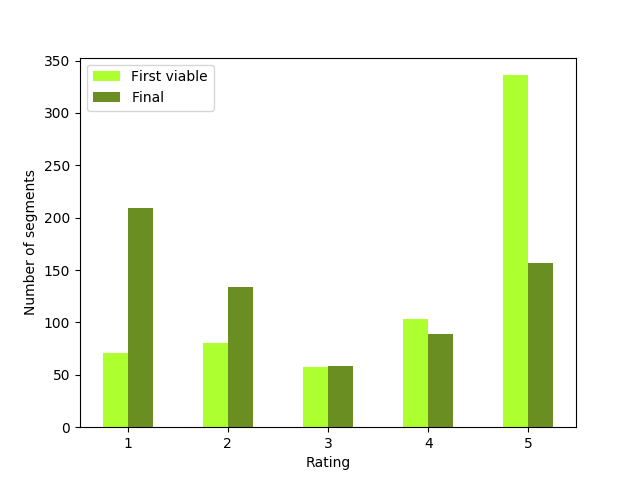
\includegraphics[width=0.8\linewidth]{img/experiment/qa_buckets.png}
    \caption{\label{fig:qa_buckets} Histogram of ratings for first viable and final translations (1 - best, 5 - worst)}
\end{figure}

The validation scores assigned to the individual segments using the histogram is presented in \cref{fig:qa_buckets}. We see that the first viable translations received mostly the worst rating while final hypotheses are bimodal: the majority received a favorable validation score but a considerable portion (24\%) had the worst score. We assume that in these cases, our setup was unreliable and fooled the user in accepting a misleading translation. A possible explanation of this is offered in \cref{sec:error_masking}.

Overall, this is a clear success, as our technique helps people to produce better messages in a language they do not speak. Nevertheless, it is important to mention the limitations of our pilot study. Our heuristics for picking first viable inputs may include sentences, which were actually not thought to be viable by the user. Maybe the sentences contained obvious errors, such as typos, which the user would fix anyway but maybe the user would not notice if we did not present the backtranslation. A more thorough exploration is needed to isolate such effects.

\subsubsection{Relation to sentence length}

One could expect that shorter sentences are generally easier to process by MT (except for very ambiguous very short sentences). To analyze this assumption in our setting, we plot the average validation score assigned to sentences based on the source length.

\begin{figure}[ht]
    \centering
    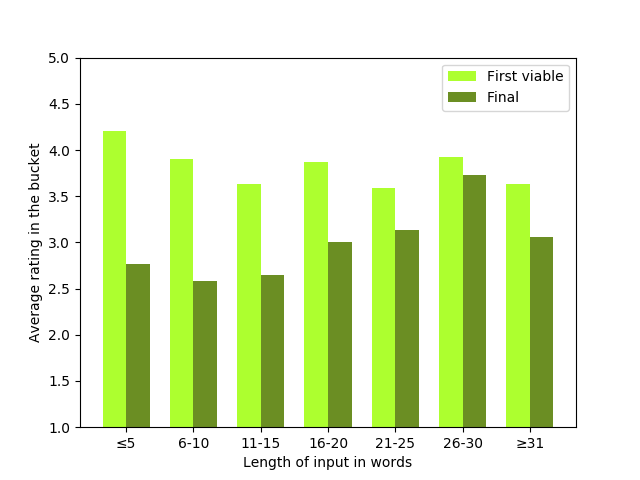
\includegraphics[width=0.8\linewidth]{img/experiment/qa_sentence_length.png}
    \caption{\label{fig:qa_sentence_length} Average rating for first viable and final translations based on the translated sentence length (1 - best, 5 - worst)}
\end{figure}

\cref{fig:qa_sentence_length} indicates that the assumed effect is not apparent in our case, at least not with our estimation of the first viable hypotheses. The shorter sentences generally receive worse validation scores than longer ones, but the differences are not very big.

For final hypotheses, the assumption seems more accurate: The best validation score was assigned to sentences of 6--10 words and the worst to sentences over 25 words. A noteworthy observation is that for these long sentences, the improvement in the validation scores from first viable to the final hypothesis is very low.

\subsection{Conclusion}

In this pilot experiment, users who did not know German were tasked to use this system for real-world use cases (communication with IT support, describing administrative issues and asking encyclopedic questions).

Across these domains, 5--10\,\% of inputs could not have been translated (our annotators have given up). For the submitted translations, the average self-reported confidence in the translations was 2.1 on a 1--5 (best--worst) scale and the tool was found more useful than standard web interfaces to MT (average usefulness of 1.71, same scale).

The majority of inputs were edited and while initial inputs and the final inputs were quite similar in the source language (word-level Gestalt Pattern Matching similarity of 75\,\%), the translations of them differed more (average similarity of 61\,\%).

The second, validation, phase of our experiment confirmed that the overall understandability of the translations improved from 3.9 to 2.71 on the 1--5 (best--worst) scale.

\pagebreak
\section{Changes in \ptakopet}
\label{sec:experiment_changes}

During the experiment, we acknowledged the need for separating experiment definitions from the rest of the code. As a result, the whole experiment content can be specified by a single JSON file instead of having to be hardcoded in the project. This is described in detail \cref{sec:experiment_def}. We also restructured the whole codebase, so that the experiment and settings profiles are more separated. The original version commit on which the pilot experiment took place got the \texttt{v-pilot} tag in the \texttt{zouharvi/ptakopet} repository.

In preparation for the next experiment we added a paraphrasing module visible in the bottom right corner in \cref{fig:experiment/stimuli_ui_new.png}

The experiment user interface also changed to accommodate better more modules and stimulus in the form of images. A stimuli is now confirmed by clicking one of the five buttons. They correspond to the confidence the user itself has of their produced texts (1 lowest -- 5 most). We added the ability to leave a note anywhere in the experiment by clicking the \text{NOTE} button below the rating scale. The progress is tracked visibly on the experiment page above the scale. This way, the annotators have a better overview of the amount of work left. All of the new features are shown in \cref{fig:experiment/stimuli_ui_new.png}.

\figcap{experiment/stimuli_ui_new.png}{Screenshot of the update \ptakopet{} interface for annotators with an image stimuli}

The baked stimuli queue is now split into blocks. They were added only for management purposes so that it is easier for users to split their work into several phases. They are notified by an alert box that they completed a block.

From the server point of view, nothing has been changed. Only the logs are now stored with \texttt{<userID>-<block>.log} scheme.
\include{content/evaluation}
\chapter*{Conclusion}
\addcontentsline{toc}{chapter}{Conclusion}

In this thesis we described the issue of outbound translation as a complement to gisting. We briefly described technologies related to machine translation quality estimation and presented a new system \ptakopet{} for both real usage and for experiments in this area.

We also conducted an experiment on human annotators, which proved that cues such as backward translation or quality estimation can increase the user's confidence in the produced translation, but also improve the final translation itself. 

We found that enhancing MT with QE improves the user experience. We expect some form of quality estimation to start appearing more in publicly available MT solutions.

\section*{Future work}
\addcontentsline{toc}{section}{Future work}

In future experiments we would like to quantitatively measure which cues are most relevant for outbound translation and how they project on user confidence in the translation. This can be done by providing different cues to different users on the same task and seeing how it affects their performance and trust in the MT system.

From the described experiment we already know that not all errors get recovered in the backward translation. This is a proof that backward translation is useful for the task of outbound translation, at least to some extent. We wish to explore this issue of backtranslation errors in general and see for example how many errors and of what kind get recovered.

Lastly we would like to explore how to gather more QE data, because at this time only a very small dataset of manually annotated QE data for several language pairs is publicly available by WMT. This QE data synthesis is a work in progress.\footnotehref{https://github.com/zouharvi/MosQEto}{github.com/zouharvi/MosQEto}

%%% Bibliography
%%% Bibliography (literature used as a source)
%%%
%%% We employ bibTeX to construct the bibliography. It processes
%%% citations in the text (e.g., the \cite{...} macro) and looks up
%%% relevant entries in the bibliography.bib file.
%%%
%%% The \bibliographystyle command selects, which style will be used
%%% for references from the text. The argument in curly brackets is
%%% the name of the corresponding style file (*.bst). Both styles
%%% mentioned in this template are included in LaTeX distributions.

\bibliographystyle{plainnat}    %% Author (year)
% \bibliographystyle{unsrt}     %% [number]

\renewcommand{\bibname}{Bibliography}

%%% Generate the bibliography. Beware that if you cited no works,
%%% the empty list will be omitted completely.

\bibliography{bibliography}

%%% If case you prefer to write the bibliography manually (without bibTeX),
%%% you can use the following. Please follow the ISO 690 standard and
%%% citation conventions of your field of research.

% \begin{thebibliography}{99}
%
% \bibitem{lamport94}
%   {\sc Lamport,} Leslie.
%   \emph{\LaTeX: A Document Preparation System}.
%   2nd edition.
%   Massachusetts: Addison Wesley, 1994.
%   ISBN 0-201-52983-1.
%
% \end{thebibliography}

\listoffigures
\listoftables
\lstlistoflistings
\addcontentsline{toc}{chapter}{List of Listings}

%%% Abbreviations used in the thesis, if any, including their explanation
%%% In mathematical theses, it could be better to move the list of abbreviations to the beginning of the thesis.
\chapwithtoc{List of Abbreviations}

\begin{description}
	
	\item[NLP] Natural Language Processing
	
	\item[RBMT, SMT, NMT] Rule Based Machine Translation, Statistical Machine Translation, Neural Machine Translation

    \item[QE] Quality Estimation
	
	\item[RTT] Round Trip Translation
	
	\item[WMT] Workshop on Statistical Machine Translation\footnotehref{http://statmt.org}{statmt.org}
	
	\item[BUCC] Workshop on Building and Using Comparable Corpora\footnotehref{https://comparable.limsi.fr}{comparable.limsi.fr}
	
	\item[SVM] Support-vector Machine, a machine learning model\footnotehref{https://en.wikipedia.org/wiki/Support-vector\_machine}{en.wikipedia.org/wiki/Support-vector\_machine}
	
	\item[W3C] World Wide Web Consortium
	
	\item[OPUS] The Open Parallel Corpus\footnotehref{http://opus.nlpl.eu/}{opus.nlpl.eu/}
	
	\item[HTER] Human-targeted Translation Error Rate - the minimum number of edits, so that the result is similar enough in meaning to the reference text
	
	\item[(bi)RNN] (bidirectional) Recurent Neural Network
	
	\item[GRU, LSTM] Gated Reccurent Units and Long Short-Term Memory are building blocks of RNN
	
\end{description}


%%% Attachments to the bachelor thesis, if any. Each attachment must be
%%% referred to at least once from the text of the thesis. Attachments
%%% are numbered.
%%%
%%% The printed version should preferably contain attachments, which can be
%%% read (additional tables and charts, supplementary text, examples of
%%% program output, etc.). The electronic version is more suited for attachments
%%% which will likely be used in an electronic form rather than read (program
%%% source code, data files, interactive charts, etc.). Electronic attachments
%%% should be uploaded to SIS and optionally also included in the thesis on a~CD/DVD.
%%% Allowed file formats are specified in provision of the rector no. 72/2017.
\appendix

\chapter{Attachments}

\section{Snapshot of \ptakopet{} frontend repository}
Besides the source code for the web application, the frontend repository contains also tools for the experiment and documentation source. The snapshot was created at \texttt{15dab17f}. It was mirrored from \href{https://github.com/zouharvi/ptakopet}{github.com/zouharvi/ptakopet}. The main repository directory structure is discussed in the technical documentation in \cref{chp:development_doc}.

\section{Snapshot of \ptakopet{} backend repository}
The backend repository, mirrored from \href{https://github.com/zouharvi/ptakopet-server}{github.com/zouharvi/ptakopet-server}, contains server code at \texttt{f099a35b}. The repository directory structure is discussed in the technical documentation in \cref{chp:development_doc}.

\section{Snapshot of SlowAlign repository}
We used SlowAlign \href{https://vilda.net/s/slowalign/}{vilda.net/s/slowalign} to produce alignment figures. It is a snapshot of \href{https://github.com/zouharvi/SlowAlign}{github.com/zouharvi/SlowAlign} at \texttt{0a158baf}.

\section{Trained models}
The attachment also contains two trained DeepQuest models, Czech$\rightarrow$German and English$\rightarrow$German and one OpenKiwi model, Czech$\rightarrow$German. They are, however, downloaded automatically when running the backend install script.

% \section{Experiment Annotation Instructions}
% The instructions for annotators in Czech are attached to this thesis in PDF.
\chapter{Development documentation}
\label{chp:development_doc}

In this appendix we aim to describe all technical details regarding the deploymend and implementation of \ptakopet{}. It is a complement to \cref{chp:implementation} which deals with the implementation.

\section{Frontend}

The \texttt{zouharvi/ptakopet} repository contains the following directory structure:

\begin{itemize}
    \item \texttt{dist/} - output directory, which contains all of the build files.
    \item \texttt{docs/} - source code for the \ptakopet{} documentation; the content is located in \texttt{docs/src/} and is written in simple markdown\footnote{Documentation is generated dynamically from the markdown by \href{https://docsify.js.org/}{docsify.js.org}.}
    \item \texttt{meta/}
        - files related to the whole project and not just the frontend
        \begin{itemize}
            \item \texttt{meta/logo} - the \ptakopet{} bird logo and relevant files
            \item \texttt{meta/object\_design} - diagrams, which describe the project workings. They are used also in the documentation
            \item \texttt{meta/study\_pilot} - all of the files connected with the pilot experiment. The contents are further described in \cref{sec:dev_doc:log_eval}
        \item \texttt{meta/synth\_qe\_test} - data and evaluation script for the experiment, which tested the quality of transferred QE data (described in \cref{subsec:cs_de_wmt})
        \end{itemize}
    \item \texttt{node\_modules/} - dependencies downloaded automatically by npm\footnotehref{https://www.npmjs.com/}{www.npmjs.com}
    \item \texttt{package.json} - the build commands and list of dependencies
    \item \texttt{package-lock.json} - list of all dependencies together with their versions in the project.
    \item \texttt{README.md} - introductory text about \ptakopet{}
    \item \texttt{src/} - source files; their structure is described in detail in \cref{sec:implementation:frontend_structure}
    \item \texttt{tsconfig.json} - TypeScript compiler settings.
    \item \texttt{webpack.config.js} - Webpack settings
\end{itemize}

\subsection{Build and compilation}

The code in \cref{lst:frontend_build_scripts} clones and builds the whole frontend in production mode:

\begin{lstlisting}[language=none, caption={Shell code for building the whole frontend},label={lst:frontend_build_scripts}]
git clone https://github.com/zouharvi/ptakopet
cd ptakopet
git submodule update --init
npm install
npm run build
\end{lstlisting}

All of the files necessary for running the frontend should then be present in the \texttt{dist/} directory. The web page does not need to be served from the Internet and can be run locally.\footnote{It still needs a server to respond to various MT related requests.} To do so, it is sufficient to load \texttt{dist/index.html} in any modern browser.

Moreover, if one wishes to rebuild the code upon every change in the source files, they may run \lstinline{npm run dev}. This starts a small HTTP server and makes the application accessible from localhost. Upon code changes, the code gets recompiled in development mode.

\subsection{Architecture}

The source files directory has the following structure:

\begin{itemize}
    \item \texttt{src/messages/} - code for anything related to backend requests (machine translation, quality estimation, alignment and paraphrasing)
    \item \texttt{src/misc/} - miscellaneous files (code utilities, current page config and profiles)
    \item \texttt{src/page/} - files relevant to DOM manipulation
    \item \texttt{src/study/} - code for displaying and collecting experiment data
    \item \texttt{src/main.ts} - entry point for the frontend application
\end{itemize}


\subsubsection*{Backends} \label{subsubsec:dev_doc:backend}

As mentioned in \cref{subsubsec:impl:backend}, a backend in this context is just an object, which contains a list of supported language pairs, a name and a function, which for some input returns a promise of the relevant output. For example in case of \texttt{Estimator} one may define a \backendname{Random} backend as in \cref{lst:random_qe}.

\begin{lstlisting}[language=none, caption={Random quality estimation backend definition},label={lst:random_qe}]
{
composeRequest(
    [lang1, lang2]: [LanguageCode, LanguageCode],
    [text1, text2]: [string, string],
    extra: ExtraTranslationInfo
): Promise<Estimation> {
    return new Promise<Estimation>(async (resolve, reject)
    => {
        let tokens = await tokenizer.tokenize(
            targetText, Settings.language2 as LanguageCode)
        let estimation: Estimation = []
        for (let i in tokens)
            estimation.push(Math.random())
        resolve(estimation)
    })
},

languages:
    Utils.generatePairsSet<LanguageCode>(Utils.Languages),

name:
    'Random'
}
\end{lstlisting}

\subsubsection{Highlighting} \label{subsubsec:dev_doc:highlighting}

As part of the quality estimation and source complexity presentation, we wanted to highlight suspicious parts of the target and source texts, respectively. Even though this seems like a trivial and prevalent task in web development, we found a lack of robust and functional solutions. Our goal was to extend the functionality of the \texttt{textarea} element so that we could display the highlighting, but keeping the user experience unaffected.

The first option we explored was based on editable \texttt{div} elements. A \texttt{div} can be made editable using the attribute \texttt{contenteditable="true"}. The \texttt{div} would then be filled by tokens, each in its \texttt{span}. The tokens could then be styled, for example with an attribute like \texttt{style='background-color: red'}. Even though this would potentially offer extensive functionality, we found it very difficult to work with. One of the biggest issues was that element focus and cursor position was lost on rerender.

The other approach, which we eventually chose, was also used in \ptakopet{}-old-2. It is based on a plugin\footnotehref{https://github.com/lonekorean/highlight-within-textarea}{github.com/lonekorean/highlight-within-textarea} by Will Boyd named highlight-within-textarea. It is a simple jQuery plugin, which uses a placeholder div (overlapping with the textarea), which is redrawn according to the current highlight values. This way, the active textarea element does not lose focus nor cursor position because it is not being manipulated. It is also beneficial that it works on mobile browsers as well.

Unfortunately, we could not use this plugin out of the box, as it was created to highlight keywords in the text. We thus forked\footnotehref{https://github.com/zouharvi/highlight-within-textarea}{github.com/zouharvi/highlight-within-textarea} this project and added the desired functionality. This project is incorporated in the main \ptakopet{} repository as a git submodule.

During the pilot experiment, we found out that there is a serious memory leak in this plugin. This did not manifest in the original plugin, as the set of keywords to highlight needed to be defined only once. For our use case, we needed to display different highlight values roughly every second. After bisecting the bug, we committed the fix into the forked repository.

\pagebreak
\section{Experiment definition} \label{sec:dev_doc:experiment_def}

In this section we describe the experiment definition on the frontend side. The tools used for generating queues and stimuli and log evaluation are discussed in \cref{sec:dev_doc:prepare_stimuli} and \cref{sec:dev_doc:log_eval}.

An experiment can be defined in a single JSON file. It is included compile-time in the \texttt{src/study/baked\_study.ts} file. The \texttt{src/study/data/} directory contains two files:
\begin{itemize}
    \item \texttt{study\_pilot.json} - definition for the experiment described in this thesis
    \item \texttt{study\_edin.json} - definition for an upcoming experiment which is part of this thesis
\end{itemize}

The JSON file has to contain a top-level object containing the keys \texttt{users}, \texttt{stimuliID} and \texttt{stimuliRules}. We explain every item type in a separate paragraph and provide a TypeScript type definition for the whole document in \cref{lst:experiment_def_type}.

\begin{lstlisting}[caption={Experiment definition type}, label={lst:experiment_def_type}, escapeinside={\%*}{*)}, stringstyle=\ttfamily, showstringspaces=false]
interface BakedStudyType {
    users: {
        [id: string]: Array<Array<string>>
    },
    stimuli: {
        [id: string]: string
    },
    stimuliRules: Array<{
        rule: string,
        message?: string,
        profile?: SettingsProfile,
    }>,
}

interface SettingsProfile {
    settings?: SettingsObject,
    qe?: boolean, // quality estimation
    mt?: boolean, // machine translation (translate 1)
    bt?: boolean, // backward translation (translate 2)
    pp?: boolean, // paraphrasing
    manual?: boolean, // allow further manual settings
}
\end{lstlisting}

\subsubsection*{\texttt{users}}

\texttt{users} is an object with \texttt{userID} keys. These keys map to an array of arrays of \texttt{stimuliIDExtended}s. This defines the experiment blocks (every innermost array is a separate block) and corresponding stimuli references. The \texttt{users} object can look like in \cref{lst:experiment_def_users}.

\begin{lstlisting}[caption={\texttt{users} experiment definition example}, label={lst:experiment_def_users}, escapeinside={\%*}{*)}, stringstyle=\ttfamily, showstringspaces=false]
"users": {
    "alice": [
        [ "003#bt.n", "007#bt.n", "012#bt.y", ... ],
        [ "020#bt.y", "011#bt.y", "050#bt.y", ... ]
    ],
    "bob": [
        [ "101#bt.n", "003#bt.y", "084#bt.n", ... ],
        [ "054#bt.n", "059#bt.y", "102#bt.n", ... ]
    ],
},
\end{lstlisting}

\subsubsection*{\texttt{stimuli}}

\texttt{stimuli} is an object with \texttt{stimuliID} keys mapping to a HTML string, which gets pasted into the page when the given stimuli is to be shown. It is important to note, that it can by any HTML, like images, not just text. The example in \cref{lst:experiment_def_stimuli} contains excerpts from stimuli of the experiment. The strings are paragraphs with \texttt{<mark>} tags which highlight parts of the shown text.

\begin{lstlisting}[caption={\texttt{stimuli} experiment definition example}, label={lst:experiment_def_stimuli}, escapeinside={\%*}{*)}, stringstyle=\ttfamily, showstringspaces=false]
"stimuli": {
    "001": "<p>A new style of wafers composed of gallium-
        nitride-on-silicon (GaN-on-Si) is being used to
        produce white LEDs using <mark>200-mm</mark>
        silicon wafers. ... </p>",
    "002": "<p>Average annual precipitation is <mark>15
        inches</mark> (380 mm), but great variations
        are seen. ... </p>",
    ...
}
\end{lstlisting}

\subsubsection*{\texttt{stimuliRules}}

\texttt{stimuliRules} is an array of \texttt{stimuliRule} objects, which contain the regex and a \texttt{settings} object. If the regex matches the current \texttt{stimulIDExtended}, the settings are applied. Multiple settings objects can be applied and can even override each other. The last rule in the array gets applied last. This allows the \texttt{stimuliIDExtended} (in the \texttt{users} section) to contain different information about e.g., whether the paraphraser should be shown to a given user, while still sharing the same \texttt{stimuliID}.

An example of a \texttt{stimuliRules} array is shown in \cref{lst:experiment_def_rules}.

\subsubsection*{\texttt{stimuliIDExtended}}

\texttt{stimuliIDExtended} is composed of two parts separated by \texttt{\#}. The first part is the actual \texttt{stimuliID} by which a lookup to this object is done, while the rest is used for any symbols, that can be later recognized by \texttt{stimuliRules}.

The string can then look like: \texttt{"003\#bt.y"} and \texttt{"003\#bt.n"}. In both of these examples, the same stimulus would be shown according to the lookup in \texttt{stimuli}, but \texttt{stimuliRules} could have two rules: \texttt{"\textbackslash d+\textbackslash \#bt\textbackslash.y"} and \texttt{"\textbackslash d+\textbackslash\#bt\textbackslash.n"} which would turn the backtranslation on and off respectively.

This example is also demonstrated in \cref{lst:experiment_def_rules}. In this example a \texttt{stimuliRule} with the regex \texttt{".*"} is used. This will match anything, so other rules will only partially override this rule in case they also match. When combined with the \texttt{users} definition in \cref{lst:experiment_def_users}, the user \texttt{alice} would be shown the stimuli \texttt{003} without backward translation and \texttt{bob} would see the same stimuli but with backward translation enabled.

\subsubsection*{\texttt{stimuliRule}}

Every \texttt{stimuliRule} object has to contain a \texttt{rule} key with the relevant regex and optionally a \texttt{settings} object or a \texttt{message} string. The later is shown above the stimuli that matches the rule. It can also contain HTML markup.

\subsubsection*{\texttt{settingsProfile} object}

\texttt{settings} objects have a type defined in \cref{lst:experiment_def_type}. It contains variables, which define whether a given module should be active or not and also the backends. The manual variable defines, whether users are allowed to change the backends themselves. It defaults to \texttt{false}.

\pagebreak
\begin{lstlisting}[caption={\texttt{stimuliRules} experiment definition example}, label={lst:experiment_def_rules}, escapeinside={\%*}{*)}, stringstyle=\ttfamily, showstringspaces=false]
"stimuliRules": [
    {
        "rule": ".*",
        "profile": {
            "settings": {
                "backendTranslator": "ufalTransformer",
                "backendEstimator": "random",
                "backendAligner": "fast_align_ubuntu",
                "language1": "en",
                "language2": "cs"
            },
            "qe": true,
            "mt": true,
            "bt": true,
            "pp": false,
            "manual": false
        },
        "message": "Translate the highlighted text in
            the provided text."
    },
    {
        "rule": ".*#.*bt\\.n.*",
        "profile": {
            "bt": false
        }
    },
    {
        "rule": ".*#.*bt\\.y.*",
        "profile": {
            "bt": true
        }
    },
    ...
]
\end{lstlisting}

\pagebreak

\section{Server backend}

The \texttt{zouharvi/ptakopet-server} repository contains several folders and files:

\begin{itemize}
    \item \texttt{align/} - models and config files for bitext alignment
    \item \texttt{data/} - data which the models make use of
    \item \texttt{install.sh} - the root install script
    \item \texttt{qe/} - models and config files for quality estimation
    \item \texttt{README.md} - an introductory text about the server
    \item \texttt{server/src/} - the server source files
    \item \texttt{server/run.sh} and \texttt{server/run\_nohup.sh} - used for launching
\end{itemize}

\subsection{Installation}

The server needs to be run on a modern UNIX machine. It was tested on Ubuntu 19.10 and Fedora 31. The installation is done via a shell script \texttt{install.sh}. It first checks whether all requirements are met. The requirements are on packages installed via pip2 and pip3 (Theano, mosestokenizer, etc.), but also on system tools (CMake, g++, tar, nohup). If all requirements are satisfied, it proceeds to launch the installation scripts for alignment, quality estimation and the server itself. According to modern development standards, the server should be dockerized. On the other hand, since only usually one instance would be running at a time, dockerizing it would be overengineering.

To run the server (on \texttt{0.0.0.0:80}), launch the \texttt{server/run.sh} script. A common practice is to connect to a remote machine via SSH and launch the server. For that, there is a script \texttt{server/run\_nohup.sh}, which disregards kill signals on user logout.

\pagebreak
\section{Experiment} \label{sec:dev_doc:experiment}

All experiment data (both preparation and collected data) are stored in \texttt{ptakopet/meta/study\_pilot}. The directory is structured as:

\begin{itemize}
    \item \texttt{logs/}
    \begin{itemize}
        \item \texttt{logs/raw} anonymized collected raw log files
        \item \texttt{logs/qe\_annotation} quality annotation of the collected data
        \item \texttt{logs/stable} contains the finished product of all processing scripts
    \end{itemize}
    \item \texttt{prepare\_questions/} scripts used to genereate stimuli and also the finished baked queues
    \item \texttt{processing\_scripts/} contains all log processing scripts
    \item \texttt{README.md} introductory text about the experiment
\end{itemize}

\subsection{Stimuli preparation} \label{sec:dev_doc:prepare_stimuli}

\subsubsection{Baked queue} \label{subsubsec:dev_doc:baked_queue}

The Python program \texttt{prepare\_questions/bake.py} contains exactly this logic. Given a number of monolingual (\texttt{--cusers}) and bilingual (\texttt{--busers}) users, it will try to distribute the stimuli from the available pool as uniformly as possible. By default the output is stored in a json file \texttt{baked.json}, but this can be changed using the \texttt{--file} argument. The seed and maximum number of stimuli per user can be specified using \texttt{--seed} and \texttt{--per\_user} respectively.

The program also prints the domain sizes for every user (important only for bilingual users), the intersection between users' baked queues and a histogram. All three sections are displayed in an example output in \cref{lst:bake_example}. Users are named from \texttt{u1}, with first being all the monolingual ones and then all the bilingual ones.

These preparatory scripts assume that the current working directory contains two dataset files. The first is \texttt{squad-train-v2.0.json}, which is available from the SQuAD 2.0 website\footnotehref{https://rajpurkar.github.io/SQuAD-explorer/}{rajpurkar.github.io/SQuAD-explorer}. The second one is the Czech translation of the same file with structure preserved. It is hosted by Matúš Žilinec\footnotehref{https://zilinec.me/dl/datasets/squad/train-cs-v2.1.json}{zilinec.me/dl/datasets/squad/train-cs-v2.1.json} and should be stored with the name of \texttt{zilinec-train-v2.1.json}.

\pagebreak
\begin{lstlisting}[language=none,caption={Example output of baked queue generator}, label={lst:bake_example}]
> ./prepare_questions/bake.py --cusers 2 --busers 2

s: SQuAD, z: SQuAD Czech, t: Tech issues, p: Praha 6
     s  z  t  p
u0: 00 60 35 30
u1: 00 60 35 30
u2: 33 27 35 30
u3: 20 40 35 30

Intersections (in %)
     u0  u1  u2  u3
u0  100 100  73  84
u1  100 100  73  84
u2   73  73 100  75
u3   84  84  75 100

Histogram: X stimuli used by Y users
31: 1, 22: 2, 31: 3, 83: 4
\end{lstlisting}

\subsubsection{Data extraction}

Stimuli for the technical and administrative domains were chosen manually. For SQuAD and SQuAD Czech, we extracted the stimuli at random using \texttt{prepare\_questions/data\_prep.py}. We used this program to explore the SQuAD structure and also to pick stimuli of interest. As described by \cref{tab:squad_distribution}, we wanted to focus on how many questions SQuAD had per given stimuli and sample within a specific distribution. When using this data extraction program with the \texttt{extract\_distribution} command, it prints the SQuAD distribution of questions per span. It also samples the spans according to the hardcoded distribution. This is shown in \cref{lst:data_prep_extraction}.

\begin{figure}[h]
\begin{lstlisting}[language=none,caption={Output of SQuAD data extraction tool}, label={lst:data_prep_extraction}, stringstyle=\ttfamily, showstringspaces=false]
> ./prepare_questions/data_prep.py \ 
    extract_distribution \ 
    output_raw.json
    
SQuAD 2.0 per span question distribution:
    {1: 81619, 2: 2303, 3: 166, 5: 8, 4: 13, 6: 1}
Total selected spans: 60
Total SQuAD 2.0 spans: 84110
\end{lstlisting}
\end{figure}

The output of this command is a JSON array, which contains tuples of the original SQuAD 2.0 and SQuAD 2.0 Czech paragraphs. For the purposes of our experiment, we also need to assign stimuli keys which we call \texttt{SID}. They are in the form of \texttt{<domain letter><number>}. The domain letters are shown in \cref{lst:bake_example}. For example the first stimuli of the SQuAD domain has \texttt{SID} of \texttt{s00}. To achieve this, we create a new JSON with the keys: \texttt{tech\_issues}, \texttt{praha\_6} and \texttt{squad}. The values for the first two are just arrays of strings and for \texttt{squad} it is the previous output. This file can then be used as an argument for the last data preparation command which adds these keys. Assuming the new edited file is stored in \texttt{all\_questions\_raw.json}, the keys can be added using as in \cref{lst:data_prep_add_keys}.

\begin{figure}[h]
\begin{lstlisting}[language=none,caption={Usage of data preparation tool command which adds \texttt{SID}s to stimuli}, label={lst:data_prep_add_keys}]
> ./prepare_questions/data_prep.py \ 
    add_keys \
    all_questions\_raw.json \
    all_questions.json
\end{lstlisting}
\end{figure}

The file \texttt{all\_questions.json} from \cref{lst:data_prep_add_keys} should now contain the JSON object which can be added to the main experiment definition file described in \cref{sec:experiment_def}.

\subsection{Logs} \label{sec:dev_doc:log_eval}

\subsubsection{Files}

The raw logs are stored in an interleaved CSV file (grepping it by the first token results in a regular CSV file). The collected files are stored with anonymized userIDs at \texttt{meta/study\_pilot/logs/raw/}. The file \texttt{meta/study\_pilot/logs/a0\_fixed.csv} contains the quality annotation of produced outputs.

\subsubsection*{Processing scripts}

For the purpose of this thesis we use files with the \texttt{.blog} extension. They simply contain pickled Python data. The logs are split into segments (each corresponding to one stimulus) and the timestamps are normalized concerning the segment's beginning. Furthermore, the lines also contain the annotator's ID.

To create the \texttt{.blog} file, use the \texttt{meta.py} command. The file can then be used by other scripts that analyze the logs. Quality estimation annotation has to be added to these files as well using the \texttt{extract\_qe\_annotation}. This process is shown in \cref{lst:data_process_blog}. We list the processing files along with their brief description:

\begin{itemize}
    \item \texttt{meta.py} aggregates all of the raw logs into a single pickled file.
    \item \texttt{domains.py} explores phenomena in segments across domains, such as the number of linearly written stimuli. 
    \item \texttt{prep\_qe\_annotation.py} creates a markdown (\texttt{qe\_annotation/a0.md}) and a CSV file which can be used by a proficient annotator to assess the quality of the produced output. We turned the markdown file into a HTML page (\texttt{qe\_annotation/a0.html}) using Pandoc.\footnotehref{https://pandoc.org/}{pandoc.org} These files were then used by this annotator and afterward, their work was merged using \texttt{extract\_qe\_annotation}. 
    \item \texttt{process\_qe\_annotation.py} processes quality annotations on collected data with graphics output which is used in this thesis and \cite{zouhar:ptakopet}. The matplotlib module is required.
    \item \texttt{segments.py} aggregates the log to some human-readable form that can be later analyzed. Examples are only written inputs (SR1) and the last translation request before confirmation (SR5). This was useful for us to examine the data.
    \item \texttt{load.py}, \texttt{create\_blog.py} and \texttt{utils.py} are used only as modules from other scripts.
\end{itemize}

\begin{lstlisting}[language=none,caption={Example of binary log file creation and manipulation}, label={lst:data_process_blog}]
> ./processing_scripts/meta.py ./logs/raw/* -b main.blog

>  ./processing_scripts/prep_qe_annotation.py ./main.blog \ 
    ./prepare_questions/questions_flat.json \ 
    --a0md a0.md --a0csv a0.csv

> ./processing_scripts/extract_qe_annotation.py \ 
    main.blog main.blog \
    ./logs/qe_annotation/a0_fixed.csv

> ./processing_scripts/domains.py ./main.blog 

SQuAD 141 (100s)
- skipped: 11
- finished: 130
- - linear: 50
- - with edits: 78
- - - avg similarity: 68.86%
- - - equal: 68.31%
- - - replace: 26.39%
- - - insert: 0.00%
- - - delete: 5.31%
SQuAD-cs 346 (94s)
- skipped: 26
- finished: 320

...

> ./processing_scripts/segments.py ./main.blog \ 
    -sr1 out.sr1 -sr2 out.sr2 -sr3 out.sr3 \
    -sr4 out.sr4 -sr5 out.sr5
\end{lstlisting}

\pagebreak
\subsubsection*{Errors} \label{subsubsec:experiment_leak}

During the experiment, we committed three mistakes. The first concerns a memory leak which made the user interface less responsive over time. This was fixed after the experiment.

The rest regards the annotation of produced translations. The second error is connected to the IDs in the CSV and HTML file given to the proficient annotator. Luckily this could be solved later by running the script \texttt{./processing\_scripts/fix\_qecsv\_usid.py ./main.blog ./logs/qe\_annotation/a0\_bad.csv ./logs/qe\_annotation/a0\_fixed.csv}. The file \texttt{a0\_bad.csv} is the one returned by the annotator and \texttt{a0\_fixed.csv} is the file with the correct mappings that can be used with other scripts.

The other error is a methodological one. The markdown/HTML file used by the annotator by which they rated the translation quality contained visible distinctions in IDs between first viable and final outputs. Since the first viable were thought to be of lesser quality, the annotator could get biased in their ratings.
\chapter{Instructions for annotators}

The following document in Czech is what was send (with minor styling edits) to the annotators from the experiment described in \cref{chp:experiment}. It briefly introduces the user interface and the annotation task with an example.

\section*{Ptakopět Pilot Experiment}

Ptakopět je nástroj pro práci s překladačem. Hlavní je levé horní textové pole, obsahující zdrojový text, pravé horní zobrazující text přeložený strojovým překladem a levé spodní, zobrazující zpětný překlad (z cizího jazyka zpět do zdrojového). První dvě zmíněná pole je možné editovat.

\begin{figure}[H]
  \centering
  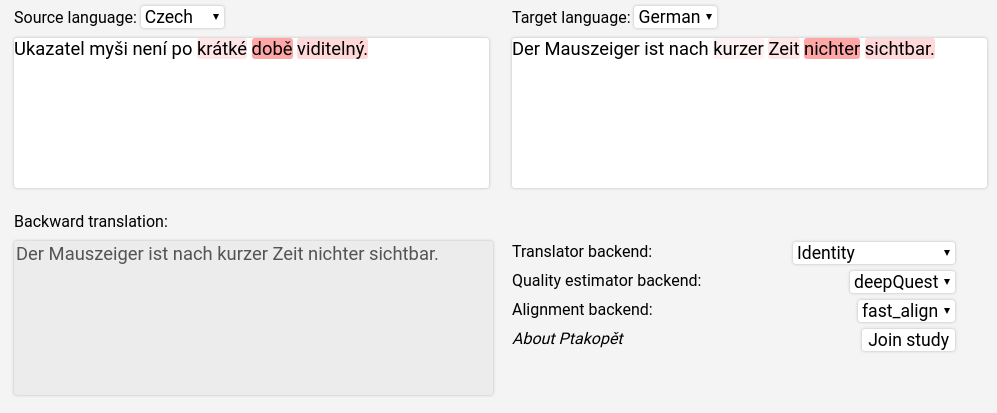
\includegraphics[width=\textwidth]{img/instructions/layout.png}
\end{figure}

Červené zabarvení v druhém poli indikuje, že překlad je v tomto místě nějakým způsobem problematický, jde ovšem o automatický odhad, který může být zavádějící. V prvním okně se pak podbarveně zobrazují slova, která pravděpodobně odpovídají těm problematickým v překladu.

\section*{Studie}

\subsection*{Úvod}

Systém je nasazen na webové adrese: \href{https://ptakopet.vilda.net/}{ptakopet.vilda.net}. Doporučujeme krátké seznámení se systémem mimo samotnou studii. V případě nejasností se, prosím, obraťte na mail \href{mailto:zouhar@ufal.mff.cuni.cz}{zouhar@ufal.mff.cuni.cz}. Studie se týká použití Ptakopětu k překladu do němčiny pro uživatele, kteří německy neumí.

Po celou dobu práce je zapotřebí být připojen k internetu. Po zmáčknutí tlačítka Join study se zobrazí dialog, do kterého je potřeba vložit vaše ID, které jste od nás dostali mailem. Pokud se vám po potvrzení zobrazí hláška Unknown user ID., bylo zadáno špatné ID a je třeba stránku načíst a zadat ID znovu.

\pagebreak

\subsection*{Příklady}

V případě úspěšného přihlášení se zobrazí první z vašich příkladů spolu s krátkou instrukcí. Ty jsou čtyř charakterů:

\begin{enumerate}
    \item Popis daného problému technické podpoře, která komunikuje pouze německy.
    \item Formulace otázky v němčině, na kterou v kontextu věty odpovídá zvýrazněná část českého odborného textu.
    \item Formulace otázky v němčině, na kterou v kontextu věty odpovídá zvýrazněná část anglického odborného textu.
    \item Formulace otázky v němčině, na kterou v kontextu věty odpovídá zvýrazněná část českého administrativního textu.
\end{enumerate}

První druh příkladu obsahuje navíc červené podbarvení, které signalizuje kvalitu překladu, ovšem ne směrodatně. Ukázka příkladu druhého druhu:

\begin{figure}[H]
  \centering
  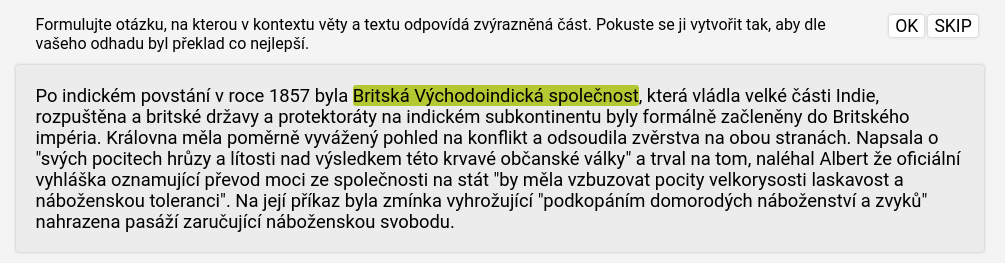
\includegraphics[width=\textwidth]{img/instructions/stimuli.png}
\end{figure}

Prvním řešením (pište do prvního textového pole) může být např. \textit{Co bylo rozpuštěno po indickém povstání v roce 1857?} Po překladu se však může ukázat, že různé obraty jsou zpětně špatně přeloženy. V takovém případě je třeba původní otázku nadále reformulovat, dokud nebudete s překladem do němčiny spokojeni (jde samozřejmě jen o váš odhad, německy neumíte).

\subsection*{Pohyb mezi příklady}

Po dokončení práce s konkrétním příkladem klikněte na tlačítko \textit{OK} a zobrazí se další. V případě, že jsou s nějakým příkladem problémy, můžete ji přeskočit tlačítkem \textit{SKIP} v takovém případě je však třeba vhodné udat důvod. Přesnější popisy jsou pro studii přínosnější.

\subsection*{Přerušení}
Váš postup je uchováván v rámci jednoho prohlížeče na jednom zařízení. Tj. zařízení i konkrétní prohlížeč lze vypínat. Po znovunačtení stránky v prohlížeči a zadání uživatelského ID by se měl zobrazit příklad, u které jste naposledy skončili. Informace o aktuálním příkladu bude ztracena v případě smazání historie, cookies, nebo dat z webu (většinou v nastavení prohlížeče).

\subsection*{Konec}

Množství otázek přesahuje váš čas pro tento projekt (zhruba 6 hodin). Až to nastane, napište mail na \href{mailto:zouhar@ufal.mff.cuni.cz}{zouhar@ufal.mff.cuni.cz}. Zde můžete buď skončit, nebo dále pokračovat, dokud nedojde zásoba otázek. Mzda je hodinová a přesný čas, který jste prací s příklady strávili se měří automaticky a ukládá na serveru.

\subsection*{Poznámka}
Během průběhu experimentu jsme stihli zaznamenat jeden technický problém. Některým uživatelům se po 5-10 minutách používání Ptakopětu snižuje responzibilita stránky Ptakopětu. Pokud se vám to stane, načtěte prosím stránku znovu.
Jedná se o technický nedostatek, který se nám bohužel na poslední chvíli nepodařilo odstranit.

\openright
\end{document}